% Options for packages loaded elsewhere
\PassOptionsToPackage{unicode}{hyperref}
\PassOptionsToPackage{hyphens}{url}
%
\documentclass[
]{book}
\usepackage{lmodern}
\usepackage{amssymb,amsmath}
\usepackage{ifxetex,ifluatex}
\ifnum 0\ifxetex 1\fi\ifluatex 1\fi=0 % if pdftex
  \usepackage[T1]{fontenc}
  \usepackage[utf8]{inputenc}
  \usepackage{textcomp} % provide euro and other symbols
\else % if luatex or xetex
  \usepackage{unicode-math}
  \defaultfontfeatures{Scale=MatchLowercase}
  \defaultfontfeatures[\rmfamily]{Ligatures=TeX,Scale=1}
\fi
% Use upquote if available, for straight quotes in verbatim environments
\IfFileExists{upquote.sty}{\usepackage{upquote}}{}
\IfFileExists{microtype.sty}{% use microtype if available
  \usepackage[]{microtype}
  \UseMicrotypeSet[protrusion]{basicmath} % disable protrusion for tt fonts
}{}
\makeatletter
\@ifundefined{KOMAClassName}{% if non-KOMA class
  \IfFileExists{parskip.sty}{%
    \usepackage{parskip}
  }{% else
    \setlength{\parindent}{0pt}
    \setlength{\parskip}{6pt plus 2pt minus 1pt}}
}{% if KOMA class
  \KOMAoptions{parskip=half}}
\makeatother
\usepackage{xcolor}
\IfFileExists{xurl.sty}{\usepackage{xurl}}{} % add URL line breaks if available
\IfFileExists{bookmark.sty}{\usepackage{bookmark}}{\usepackage{hyperref}}
\hypersetup{
  pdftitle={Collaborative Data Science Practices},
  pdfauthor={Will Beasley},
  hidelinks,
  pdfcreator={LaTeX via pandoc}}
\urlstyle{same} % disable monospaced font for URLs
\usepackage{color}
\usepackage{fancyvrb}
\newcommand{\VerbBar}{|}
\newcommand{\VERB}{\Verb[commandchars=\\\{\}]}
\DefineVerbatimEnvironment{Highlighting}{Verbatim}{commandchars=\\\{\}}
% Add ',fontsize=\small' for more characters per line
\usepackage{framed}
\definecolor{shadecolor}{RGB}{248,248,248}
\newenvironment{Shaded}{\begin{snugshade}}{\end{snugshade}}
\newcommand{\AlertTok}[1]{\textcolor[rgb]{0.94,0.16,0.16}{#1}}
\newcommand{\AnnotationTok}[1]{\textcolor[rgb]{0.56,0.35,0.01}{\textbf{\textit{#1}}}}
\newcommand{\AttributeTok}[1]{\textcolor[rgb]{0.77,0.63,0.00}{#1}}
\newcommand{\BaseNTok}[1]{\textcolor[rgb]{0.00,0.00,0.81}{#1}}
\newcommand{\BuiltInTok}[1]{#1}
\newcommand{\CharTok}[1]{\textcolor[rgb]{0.31,0.60,0.02}{#1}}
\newcommand{\CommentTok}[1]{\textcolor[rgb]{0.56,0.35,0.01}{\textit{#1}}}
\newcommand{\CommentVarTok}[1]{\textcolor[rgb]{0.56,0.35,0.01}{\textbf{\textit{#1}}}}
\newcommand{\ConstantTok}[1]{\textcolor[rgb]{0.00,0.00,0.00}{#1}}
\newcommand{\ControlFlowTok}[1]{\textcolor[rgb]{0.13,0.29,0.53}{\textbf{#1}}}
\newcommand{\DataTypeTok}[1]{\textcolor[rgb]{0.13,0.29,0.53}{#1}}
\newcommand{\DecValTok}[1]{\textcolor[rgb]{0.00,0.00,0.81}{#1}}
\newcommand{\DocumentationTok}[1]{\textcolor[rgb]{0.56,0.35,0.01}{\textbf{\textit{#1}}}}
\newcommand{\ErrorTok}[1]{\textcolor[rgb]{0.64,0.00,0.00}{\textbf{#1}}}
\newcommand{\ExtensionTok}[1]{#1}
\newcommand{\FloatTok}[1]{\textcolor[rgb]{0.00,0.00,0.81}{#1}}
\newcommand{\FunctionTok}[1]{\textcolor[rgb]{0.00,0.00,0.00}{#1}}
\newcommand{\ImportTok}[1]{#1}
\newcommand{\InformationTok}[1]{\textcolor[rgb]{0.56,0.35,0.01}{\textbf{\textit{#1}}}}
\newcommand{\KeywordTok}[1]{\textcolor[rgb]{0.13,0.29,0.53}{\textbf{#1}}}
\newcommand{\NormalTok}[1]{#1}
\newcommand{\OperatorTok}[1]{\textcolor[rgb]{0.81,0.36,0.00}{\textbf{#1}}}
\newcommand{\OtherTok}[1]{\textcolor[rgb]{0.56,0.35,0.01}{#1}}
\newcommand{\PreprocessorTok}[1]{\textcolor[rgb]{0.56,0.35,0.01}{\textit{#1}}}
\newcommand{\RegionMarkerTok}[1]{#1}
\newcommand{\SpecialCharTok}[1]{\textcolor[rgb]{0.00,0.00,0.00}{#1}}
\newcommand{\SpecialStringTok}[1]{\textcolor[rgb]{0.31,0.60,0.02}{#1}}
\newcommand{\StringTok}[1]{\textcolor[rgb]{0.31,0.60,0.02}{#1}}
\newcommand{\VariableTok}[1]{\textcolor[rgb]{0.00,0.00,0.00}{#1}}
\newcommand{\VerbatimStringTok}[1]{\textcolor[rgb]{0.31,0.60,0.02}{#1}}
\newcommand{\WarningTok}[1]{\textcolor[rgb]{0.56,0.35,0.01}{\textbf{\textit{#1}}}}
\usepackage{longtable,booktabs}
% Correct order of tables after \paragraph or \subparagraph
\usepackage{etoolbox}
\makeatletter
\patchcmd\longtable{\par}{\if@noskipsec\mbox{}\fi\par}{}{}
\makeatother
% Allow footnotes in longtable head/foot
\IfFileExists{footnotehyper.sty}{\usepackage{footnotehyper}}{\usepackage{footnote}}
\makesavenoteenv{longtable}
\usepackage{graphicx}
\makeatletter
\def\maxwidth{\ifdim\Gin@nat@width>\linewidth\linewidth\else\Gin@nat@width\fi}
\def\maxheight{\ifdim\Gin@nat@height>\textheight\textheight\else\Gin@nat@height\fi}
\makeatother
% Scale images if necessary, so that they will not overflow the page
% margins by default, and it is still possible to overwrite the defaults
% using explicit options in \includegraphics[width, height, ...]{}
\setkeys{Gin}{width=\maxwidth,height=\maxheight,keepaspectratio}
% Set default figure placement to htbp
\makeatletter
\def\fps@figure{htbp}
\makeatother
\setlength{\emergencystretch}{3em} % prevent overfull lines
\providecommand{\tightlist}{%
  \setlength{\itemsep}{0pt}\setlength{\parskip}{0pt}}
\setcounter{secnumdepth}{5}
\usepackage{booktabs}
\usepackage[]{natbib}
\bibliographystyle{apalike}

\title{Collaborative Data Science Practices}
\author{Will Beasley}
\date{2019-12-20}

\begin{document}
\frontmatter
\maketitle

{
\setcounter{tocdepth}{1}
\tableofcontents
}
\mainmatter
\hypertarget{intro}{%
\chapter{Introduction}\label{intro}}

This collection of documents describe practices used by the OUHSC \href{https://ouhsc.edu/bbmc}{BBMC} in our analytics projects.

\hypertarget{coding}{%
\chapter{Coding Principles}\label{coding}}

\hypertarget{simplify}{%
\section{Simplify}\label{simplify}}

\hypertarget{data-types}{%
\subsection{Data Types}\label{data-types}}

Use the simplest data type reasonable. A simpler data type is less likely contain unintented values. As we have seen, a string variable called \texttt{gender} can simulatneously contain the values ``m'', ``f'', ``F'', ``Female'', ``MALE'', ``0'', ``1'', ``2'', ``Latino'', "", and \texttt{NA}. On the other hand, a boolean variable \texttt{gender\_male} can be only \texttt{FALSE}, \texttt{TRUE}, and \texttt{NA}.\footnote{The database \texttt{bit} equivalents are \texttt{0}, \texttt{1}, and \texttt{NULL}}.

Once you have cleaned a variable in your initial ETL files (like an Ellis), lock it down so you do not have to spend time in the downstream files verifying that no bad values have been introduced. As a small bonus, simpler data types are typically faster, consume less memory, and translate more cleanly across platforms.

Within R, the preference for numeric-ish variables is

\begin{enumerate}
\def\labelenumi{\arabic{enumi}.}
\tightlist
\item
  \texttt{logical}/boolean/bit,
\item
  \texttt{integer},
\item
  \texttt{bit64::integer64}, and
\item
  \texttt{numeric}/double-precision floats.
\end{enumerate}

The preference for categorical variables is

\begin{enumerate}
\def\labelenumi{\arabic{enumi}.}
\tightlist
\item
  \texttt{logical}/boolean/bit,
\item
  \texttt{factor}, and
\item
  \texttt{character}.
\end{enumerate}

\hypertarget{categorical-levels}{%
\subsection{Categorical Levels}\label{categorical-levels}}

When a boolean variable would be too restrictive and a factor or character is required, choose the simplest representation. Where possible:

\begin{enumerate}
\def\labelenumi{\arabic{enumi}.}
\tightlist
\item
  Use only lower case (\emph{e.g.}, `male' instead of `Male' for the \texttt{gender} variable).
\item
  avoid repeating the variable in the level (\emph{e.g.}, `control' instead of `control condition' for the \texttt{condition} variable).
\end{enumerate}

\hypertarget{recoding}{%
\subsection{Recoding}\label{recoding}}

Almost every project recodes many variables. Choose the simplest function possible. The functions at the top are much easier to read and harder to mess up.

\begin{enumerate}
\def\labelenumi{\arabic{enumi}.}
\item
  \texttt{!}: instead of \texttt{gender\_male\ ==\ FALSE} or \texttt{gender\_male\ !=\ TRUE}, write \texttt{!gender\_male}.
\item
  \texttt{dplyr::coalesce()}: The function evaluates a single variable and replaces \texttt{NA} with values from another variable.

  A coalesce like

\begin{Shaded}
\begin{Highlighting}[]
\NormalTok{visit\_completed =}\StringTok{ }\NormalTok{dplyr}\OperatorTok{::}\KeywordTok{coalesce}\NormalTok{(visit\_completed, }\OtherTok{FALSE}\NormalTok{)}
\end{Highlighting}
\end{Shaded}

  is much easier to read and not mess up than

\begin{Shaded}
\begin{Highlighting}[]
\NormalTok{visit\_completed =}\StringTok{ }\NormalTok{dplyr}\OperatorTok{::}\KeywordTok{if\_else}\NormalTok{(}\OperatorTok{!}\KeywordTok{is.na}\NormalTok{(visit\_completed), visit\_completed, }\OtherTok{FALSE}\NormalTok{)}
\end{Highlighting}
\end{Shaded}
\item
  \texttt{\textless{}=} (or a similar comparison operator): Compare two quantities to output a boolean variable.
\item
  \texttt{dplyr::if\_else()}: The function evaluates a single boolean variable. The output branches to only three possiblities: condition is (a) true, (b) false, or (c) (optionally) \texttt{NA}. An advantage over \texttt{\textless{}=} is that \texttt{NA} values can be specified directly.

  `\texttt{month} element needs to be handled explicitly.
  stage = dplyr::if\_else(date\_start \textless= month, ``pre'', ``post'', missing = ``missing-month''),

  \# Otherwise a simple boolean output is sufficient.
  stage\_post = (date\_start \textless= month)
  ```
\item
  \texttt{base::cut()}: The function evaluations only a single numeric variable. It's range is cut into different segments/categories on the one-dimensional number line. The output branches to single discrete value (either a factor-level or an integer).
\item
  \texttt{dplyr::recode()}: The function evaluates a single integer or character variable. The output branches to a single discrete value.
\item
  \emph{lookup table}: It feasible recode 6 levels of race directly in R. It's less feasible to recode 200 provider names. Specify the mapping in a csv, \texttt{readr} the csv to a data.frame, and left-join it.
\item
  \texttt{dplyr::case\_when()}: The function is the most complicated because it can evaluate multiple variables. Also, multiple cases can be true, but only the first output is returned. This `water fall' execution helps in complicated scenarios, but is overkill for most.
\end{enumerate}

\hypertarget{defensive-style}{%
\section{Defensive Style}\label{defensive-style}}

\hypertarget{qualify-functions}{%
\subsection{Qualify functions}\label{qualify-functions}}

Try to prepend each function with its package. Write \texttt{dplyr::filter()} instead of \texttt{filter()}. When two packages contain public functions with the same name, the package that was most recently called with \texttt{library()} takes precedent. When multiple R files are executed, the packages' precedents may not be predictable. Specifying the package eliminates the ambiguity, while also making the code easier to follow. For this reason, we recommend that almost all R files contain a \protect\hyperlink{chunk-load-packages}{`load-packages'} chunk.

\hypertarget{architecture}{%
\chapter{Architecture Principles}\label{architecture}}

\hypertarget{encapsulation}{%
\section{Encapsulation}\label{encapsulation}}

\hypertarget{leverage-team-members-strenghts-avoid-weaknesses}{%
\section{Leverage team member's strenghts \& avoid weaknesses}\label{leverage-team-members-strenghts-avoid-weaknesses}}

\hypertarget{focused-code-files}{%
\subsection{Focused code files}\label{focused-code-files}}

\hypertarget{metadata-for-content-experts}{%
\subsection{Metadata for content experts}\label{metadata-for-content-experts}}

\hypertarget{scales}{%
\section{Scales}\label{scales}}

\hypertarget{single-source-single-analysis}{%
\subsection{Single source \& single analysis}\label{single-source-single-analysis}}

\hypertarget{multiple-sources-multiple-analyses}{%
\subsection{Multiple sources \& multiple analyses}\label{multiple-sources-multiple-analyses}}

\hypertarget{architecture-consistency}{%
\section{Consistency}\label{architecture-consistency}}

\hypertarget{consistency-files}{%
\subsection{Across Files}\label{consistency-files}}

\hypertarget{across-languages}{%
\subsection{Across Languages}\label{across-languages}}

\hypertarget{across-projects}{%
\subsection{Across Projects}\label{across-projects}}

\hypertarget{file-prototype}{%
\chapter{Prototypical File}\label{file-prototype}}

As stated before, in \protect\hyperlink{consistency-files}{Consistency across Files}, using a consistent file structure can (a) improve the quality of the code because the structure has been proven over time to facilitate good practices and (b) allow your intentions to be more clear to teammates because they are familiar with the order and intentions of the chunks.

We use the term ``chunk'' for a section of code because it corresponds with knitr terminology \citep{xie2015}, and in many analysis files (as opposed to manipulation files), the chunk of our R file connects to a knitr Rmd file.

\hypertarget{chunk-clear}{%
\section{Clear Memory}\label{chunk-clear}}

Before the initial chunk many of our files clear the memory of variables from previous run. This is important when developig and debugging because it prevents previous runs from contaminating subsequent runs. However it has little effect during production; we'll look at manipulation files separately from analysis files.

Manipulation R files are \href{https://stat.ethz.ch/R-manual/R-devel/library/base/html/source.html}{\texttt{source}}d with the argument \texttt{local=new.env()}. The file is executed in a fresh environment, so there are no variables to clear. Analysis R files are typically called from an Rmd file's \texttt{knitr::read\_chunk()}, and code positioned above the first chunk is not called by knitr \footnote{Read more about knitr's \href{https://yihui.name/knitr/demo/externalization/}{code externalization}}.

However typically do not clear the memory in R files that are \href{https://stat.ethz.ch/R-manual/R-devel/library/base/html/source.html}{\texttt{source}}d in the same environment as the caller, as it will interfere with the caller's variables.

\begin{Shaded}
\begin{Highlighting}[]
\KeywordTok{rm}\NormalTok{(}\DataTypeTok{list =} \KeywordTok{ls}\NormalTok{(}\DataTypeTok{all.names =} \OtherTok{TRUE}\NormalTok{))}
\end{Highlighting}
\end{Shaded}

\hypertarget{chunk-load-sources}{%
\section{Load Sources}\label{chunk-load-sources}}

In the first true chunk, \href{https://stat.ethz.ch/R-manual/R-devel/library/base/html/source.html}{\texttt{source}} any R files containing global variables and functions that the current file requires. For instance, when a team of statisticians is producing a large report containing many analysis files, we define many of the graphical elements in a single file. This sourced file defines common color palettes and graphical functions so the cosmetics are more uniform across analyses.

We prefer not to have \texttt{source}d files perform any real action, such as importing data or manipulating a file. One reason is because it is difficult to be consistent about the environmental variables when the sourced file's functions are run. A second reason is that it more cognitively difficult to understand how the files are connected.

When the sourced file contains only function definitions, these operations can be called at any time in the current file with much tighter control of which variables are modfied. A bonus of the discipline of defining functions (instead of executing functions) is that the operations are typically more robust and generalizable.

Keep the chunk even if no files are sourced. An empty chunk is instructive to readers trying to determine if any files are sourced. This applies recommendation applies to all the chunks discussed in this chapter. As always, your team should agree on its own set of standards.

\begin{Shaded}
\begin{Highlighting}[]
\CommentTok{\# {-}{-}{-}{-} load{-}sources {-}{-}{-}{-}{-}{-}{-}{-}{-}{-}{-}{-}{-}{-}{-}{-}{-}{-}{-}{-}{-}{-}{-}{-}{-}{-}{-}{-}{-}{-}{-}{-}{-}{-}{-}{-}{-}{-}{-}{-}{-}{-}{-}{-}{-}{-}{-}{-}{-}{-}{-}{-}{-}{-}{-}{-}{-}{-}{-}{-}}
\NormalTok{base}\OperatorTok{::}\KeywordTok{source}\NormalTok{(}\DataTypeTok{file=}\StringTok{"./analysis/common/display{-}1.R"}\NormalTok{)      }\CommentTok{\# Load common graphing functions.}
\end{Highlighting}
\end{Shaded}

\hypertarget{chunk-load-packages}{%
\section{Load Packages}\label{chunk-load-packages}}

The `load-packages' chunk declares required packages near the file's beginning for three reasons. First, a reader scanning the file can quickly determine its dependencies when located in a single chunk. Second, if your machine is lacking a required package, it is best to know early\footnote{The error message ``Error in library(foo) : there is no package called `foo'\,'' is easier to understand than ``Error in bar() : could not find function `bar'\,'' thrown somewhere in the middle of the file; this check can also illuminate conflicts arising when two packages have a \texttt{bar()} function. See McConnell 2004 Section qqq for more about the `fail early' principle.}. Third, this style mimics a requirement of other languages (such as declaring headers at the top of a C++ file) and follows the \href{https://style.tidyverse.org/files.html\#internal-structure}{tidyverse style guide}.

As discussed in the previous \protect\hyperlink{qualify-functions}{qualify all functions} section, we recommend that functions are qualified with their package (\emph{e.g.}, \texttt{foo::bar()} instead of merely \texttt{bar()}). Consequently, the `load-packages' chunk calls \texttt{requireNamespace()} more frequently than \texttt{library()}. \texttt{requireNamespace()} verifies the package is available on the local machine, but does not load it into memory; \texttt{library()} verifies the package is available, and then loads it.

\texttt{requireNamespace()} is not used in several scenarios.

\begin{enumerate}
\def\labelenumi{\arabic{enumi}.}
\tightlist
\item
  Core packages (\emph{e.g.}, `base' and `stats') are loaded by R in most default installations. We avoid unnecessary calls like \texttt{library(stats)} because they distract from more important features.
\item
  Obvious dependencies are not called by \texttt{reqiureNamespace()} or \texttt{library()} for similar reasons, especially if they are not called directly. For example `tidyselect' is not listed when `tidyr' is listed.
\item
  The ``pipe'' function (declared in the \texttt{magrittr\textquotesingle{}\ package\ ,\ *i.e.*,}\%\textgreater\%\texttt{)\ is\ attached\ with}import::from(magrittr, ``\%\textgreater\%'')`. This frequently-used function called be called throughout the execution without qualification.
\item
  Compared to manipulation files, our analysis files tend to use many functions in a few concentrated packages so conflicting function names are less common. Typical packages used in analysis are `ggplot2' and `lme4'.
\end{enumerate}

The \texttt{source}d files above may load their own packages (by calling \texttt{library()}). It is important that the \texttt{library()} calls in this file follow the `load-sources' chunk so that identically-named functions (in different packages) are called with the correct precedent. Otherwise identically-named functions will conflict in the namespace with hard-to-predict results.

Read \href{http://r-pkgs.had.co.nz/namespace.html\#search-path}{R Packages} for more about \texttt{library()}, \texttt{requireNamespace()}, and their siblings, as well as the larger concepts such as attaching functions into the search path.

Here are packages found in most of our manipulation files. Notice the lesser-known packages have a quick explanation; this helps maintainers decide if the declaration is still necessary. Also notice the packages distributed outside of CRAN (\emph{e.g.}, GitHub) have a quick commented line to help the user install or update the package.

\begin{Shaded}
\begin{Highlighting}[]
\CommentTok{\# {-}{-}{-}{-} load{-}packages {-}{-}{-}{-}{-}{-}{-}{-}{-}{-}{-}{-}{-}{-}{-}{-}{-}{-}{-}{-}{-}{-}{-}{-}{-}{-}{-}{-}{-}{-}{-}{-}{-}{-}{-}{-}{-}{-}{-}{-}{-}{-}{-}{-}{-}{-}{-}{-}{-}{-}{-}{-}{-}{-}{-}{-}{-}{-}{-}}
\NormalTok{import}\OperatorTok{::}\KeywordTok{from}\NormalTok{(magrittr, }\StringTok{"\%>\%"}\NormalTok{ )}

\KeywordTok{requireNamespace}\NormalTok{(}\StringTok{"readr"}\NormalTok{     )}
\KeywordTok{requireNamespace}\NormalTok{(}\StringTok{"tidyr"}\NormalTok{     )}
\KeywordTok{requireNamespace}\NormalTok{(}\StringTok{"dplyr"}\NormalTok{     ) }
\KeywordTok{requireNamespace}\NormalTok{(}\StringTok{"config"}\NormalTok{    ) }
\KeywordTok{requireNamespace}\NormalTok{(}\StringTok{"checkmate"}\NormalTok{ ) }\CommentTok{\# Asserts expected conditions }
\KeywordTok{requireNamespace}\NormalTok{(}\StringTok{"OuhscMunge"}\NormalTok{) }\CommentTok{\# remotes::install\_github(repo="OuhscBbmc/OuhscMunge")}
\end{Highlighting}
\end{Shaded}

\hypertarget{chunk-declare}{%
\section{Declare Globals}\label{chunk-declare}}

When values are repeatedly used within a file, consider dedicating a variable so it's defined and set only once. This is also a good place for variables that are used only once, but whose value are central to the file's mission. Typical variables in our `declare-globals' chunk include data file paths, data file variables, color palettes, and values in the \emph{config} file.

The \protect\hyperlink{repo-root}{config file} can coordinate a static variable across multiple files. Centrally

\begin{Shaded}
\begin{Highlighting}[]
\CommentTok{\# {-}{-}{-}{-} declare{-}globals {-}{-}{-}{-}{-}{-}{-}{-}{-}{-}{-}{-}{-}{-}{-}{-}{-}{-}{-}{-}{-}{-}{-}{-}{-}{-}{-}{-}{-}{-}{-}{-}{-}{-}{-}{-}{-}{-}{-}{-}{-}{-}{-}{-}{-}{-}{-}{-}{-}{-}{-}{-}{-}{-}{-}{-}{-}}
\CommentTok{\# Constant values that won\textquotesingle{}t change.}
\NormalTok{config                         <{-}}\StringTok{ }\NormalTok{config}\OperatorTok{::}\KeywordTok{get}\NormalTok{()}
\NormalTok{path\_db                        <{-}}\StringTok{ }\NormalTok{config}\OperatorTok{$}\NormalTok{path\_database}

\CommentTok{\# Execute to specify the column types.  It might require some manual adjustment (eg doubles to integers).}
\CommentTok{\#   OuhscMunge::readr\_spec\_aligned(config$path\_subject\_1\_raw)}
\NormalTok{col\_types <{-}}\StringTok{ }\NormalTok{readr}\OperatorTok{::}\KeywordTok{cols\_only}\NormalTok{(}
  \DataTypeTok{subject\_id          =}\NormalTok{ readr}\OperatorTok{::}\KeywordTok{col\_integer}\NormalTok{(),}
  \DataTypeTok{county\_id           =}\NormalTok{ readr}\OperatorTok{::}\KeywordTok{col\_integer}\NormalTok{(),}
  \DataTypeTok{gender\_id           =}\NormalTok{ readr}\OperatorTok{::}\KeywordTok{col\_double}\NormalTok{(),}
  \DataTypeTok{race                =}\NormalTok{ readr}\OperatorTok{::}\KeywordTok{col\_character}\NormalTok{(),}
  \DataTypeTok{ethnicity           =}\NormalTok{ readr}\OperatorTok{::}\KeywordTok{col\_character}\NormalTok{()}
\NormalTok{)}
\end{Highlighting}
\end{Shaded}

\hypertarget{chunk-load-data}{%
\section{Load Data}\label{chunk-load-data}}

All data ingested by this file occurs in this chunk. We like to think of each file as a linear pipe with a single point of input and single point of output. Although it is possible for a file to read data files on any line, we recommend avoiding this sprawl because it is more difficult for humans to understand. If the software developer is a deist watchmaker, the file's fate has been sealed by the end of this chunk. This makes is easier for a human to reason to isolate problems as either existing with (a) the incoming data or (b) the calculations on that data.

Ideally this chunk consumes data from either a plain-text csv or a database.

Many capable R functions and packages ingest data. We prefer the tidyverse \href{https://readr.tidyverse.org/}{readr} for reading conventional files; its younger cousin, \href{}{vroom}\url{https://vroom.r-lib.org/} has some nice advantages when working with larger files and some forms of jagged rectangles\footnote{Say a csv has 20 columns, but a row has missing values for the last five columns. Instead of five successive commas to indicate five empty cells exist, a jagged rectangle simply ends after the last nonmissing value. vroom infers the missing values correctly, while some other packages do not.}. Depending on the file format, good packages to consider are \href{https://cran.r-project.org/package=data.table}{data.table}, \href{https://haven.tidyverse.org/}{haven}, \href{https://readxl.tidyverse.org/}{readxl}, \href{https://ycphs.github.io/openxlsx/}{openxlsx}, \href{https://CRAN.R-project.org/package=arrow}{arrow}, \href{https://CRAN.R-project.org/package=jsonlite}{jsonlite}, \href{http://www.fstpackage.org/}{fst}, \href{https://CRAN.R-project.org/package=yaml}{yaml}, and \href{https://cloud.r-project.org/web/packages/rio/vignettes/rio.html}{rio}.

When used in an \protect\hyperlink{pattern-ellis}{Ellis}, this chunk likely consumees a flat file like a csv with data or metadata. When used in a \protect\hyperlink{pattern-ferry}{Ferry}, \protect\hyperlink{pattern-arch}{Arch}, or \protect\hyperlink{pattern-scribe}{Scribe}, this chunk likely consumes a database table. When used in an \protect\hyperlink{pattern-analysis}{Analysis file}, this chunk likely cosumes a database table or rds (\emph{i.e.}, a compressed R data file).

In some large-scale scenarios, there may be a series of datasets that cannot be held in RAM simultaneously. Our first choice is to split the R file so each new file has only a subset of the datasets --in other words, the R file probably was given too much responsibility. Occassionaly the multiple datasets need to be considered at once, so splitting the R file is not a option. In these scenarios, we prefer to upload all the datasets to a database, which is better manipulating datasets too large for RAM.

An R solution may be to losen the restriction that dataset enter the R file only during the `load-data' chunk. Once a dataset is processed and no longer needed, \texttt{rm()} \emph{r}e\emph{m}oves it from RAM. Now another dataset can be read from a file and manipulated.

\emph{loose scrap}:
the chunk reads all data (\emph{e.g.}, database table, networked CSV, local lookup table). After this chunk, no new data should be introduced. This is for the sake of reducing human cognition load. Everything below this chunk is derived from these first four chunks.

\hypertarget{tweak-data-chunk-tweak-data}{%
\section{Tweak Data (\#chunk-tweak-data)}\label{tweak-data-chunk-tweak-data}}

\emph{loose scrap}:
It's best to rename the dataset (a) in a single place and (b) early in the pipeline, so the bad variable are never referenced.

\begin{Shaded}
\begin{Highlighting}[]
\CommentTok{\# OuhscMunge::column\_rename\_headstart(ds) \# Help write \textasciigrave{}dplyr::select()\textasciigrave{} call.}
\NormalTok{ds <{-}}
\StringTok{  }\NormalTok{ds }\OperatorTok{\%>\%}
\StringTok{  }\NormalTok{dplyr}\OperatorTok{::}\KeywordTok{select}\NormalTok{(    }\CommentTok{\# \textasciigrave{}dplyr::select()\textasciigrave{} drops columns not included.}
\NormalTok{    subject\_id,}
\NormalTok{    county\_id,}
\NormalTok{    gender\_id,}
\NormalTok{    race,}
\NormalTok{    ethnicity}
\NormalTok{  ) }\OperatorTok{\%>\%}
\StringTok{  }\NormalTok{dplyr}\OperatorTok{::}\KeywordTok{mutate}\NormalTok{(}

\NormalTok{  )  }\OperatorTok{\%>\%}
\StringTok{  }\NormalTok{dplyr}\OperatorTok{::}\KeywordTok{arrange}\NormalTok{(subject\_id) }\CommentTok{\# \%>\%}
  \CommentTok{\# tibble::rowid\_to\_column("subject\_id") \# Add a unique index if necessary}
\end{Highlighting}
\end{Shaded}

\hypertarget{chunk-unique}{%
\section{(Unique Content)}\label{chunk-unique}}

This section represents all the chunks between \protect\hyperlink{chunk-tweak-data}{tweak-data} and \protect\hyperlink{chunk-verify-values}{verify-values}. These chunks contain most of of the file's creativity and contribution. In a sense, the structure of the first and last chunks allow these middle chunks to focus on concepts instead of plumbing.

For simple files like the ellis of a metadata file, may not even need anything here. But complex analysis files may have 200+ lines distributed across a dozen chunks. We recommend that you create dedicate a chunk to each conceptual stage. If one starts to contain more than \textasciitilde20 lines, consider if a more granular organization would clarify the code's intent.

\hypertarget{chunk-verify-values}{%
\section{Verify Values}\label{chunk-verify-values}}

Running \texttt{OuhscMunge::verify\_value\_headstart(ds)} will

\begin{verbatim}
```r
# ---- verify-values -----------------------------------------------------------
# Sniff out problems
# OuhscMunge::verify_value_headstart(ds)
checkmate::assert_integer(  ds$county_month_id    , any.missing=F , lower=1, upper=3080                , unique=T)
checkmate::assert_integer(  ds$county_id          , any.missing=F , lower=1, upper=77                            )
checkmate::assert_date(     ds$month              , any.missing=F , lower=as.Date("2012-06-15"), upper=Sys.Date())
checkmate::assert_character(ds$county_name        , any.missing=F , pattern="^.{3,12}$"                          )
checkmate::assert_integer(  ds$region_id          , any.missing=F , lower=1, upper=20                            )
checkmate::assert_numeric(  ds$fte                , any.missing=F , lower=0, upper=40                            )
checkmate::assert_logical(  ds$fte_approximated   , any.missing=F                                                )
checkmate::assert_numeric(  ds$fte_rolling_median , any.missing=T , lower=0, upper=40                            )

county_month_combo   <- paste(ds$county_id, ds$month)
checkmate::assert_character(county_month_combo, pattern  ="^\\d{1,2} \\d{4}-\\d{2}-\\d{2}$", any.missing=F, unique=T)
```
\end{verbatim}

\hypertarget{chunk-specify-columns}{%
\section{Specify Output Columns}\label{chunk-specify-columns}}

This chunk:

\begin{enumerate}
\def\labelenumi{\arabic{enumi}.}
\tightlist
\item
  verifies these variables exist before uploading,
\item
  documents (to troubleshooting developers) these variables are a product of the file, and
\item
  reorders the variables to match the expected structure.
\end{enumerate}

Variable order is especially important for the database engines/drivers that ignore the variable name, and use only the variable position.

We use the term `slim' because typically this output has fewer variables than the full dataset processed by the file.

If you doubt the variable will be needed downstream, leave it in the \texttt{dplyr::select()}, but commented out. If someone needs it in the future, they'll easily determine where it might come from, and then uncomment the line (and possibly modify the database table). Once you import a column into a warehouse that multiple people are using, it can be tough to remove without breaking their code.

This chunk follows \protect\hyperlink{chunk-verify-values}{verify-values} because sometimesyou want to check the validity of variables that are not consumed downstream. These variables are not important themselves, but an illegal value may reveal a larger problem with the dataset.

\begin{Shaded}
\begin{Highlighting}[]
\CommentTok{\# Print colnames that \textasciigrave{}dplyr::select()\textasciigrave{}  should contain below:}
\CommentTok{\#   cat(paste0("    ", colnames(ds), collapse=",\textbackslash{}n"))}

\CommentTok{\# Define the subset of columns that will be needed in the analyses.}
\CommentTok{\#   The fewer columns that are exported, the fewer things that can break downstream.}

\NormalTok{ds\_slim <{-}}
\StringTok{  }\NormalTok{ds }\OperatorTok{\%>\%}
\StringTok{  }\CommentTok{\# dplyr::slice(1:100) \%>\%}
\StringTok{  }\NormalTok{dplyr}\OperatorTok{::}\KeywordTok{select}\NormalTok{(}
\NormalTok{    subject\_id,}
\NormalTok{    county\_id,}
\NormalTok{    gender\_id,}
\NormalTok{    race,}
\NormalTok{    ethnicity}
\NormalTok{  )}

\NormalTok{ds\_slim}
\end{Highlighting}
\end{Shaded}

\hypertarget{save-to-disk-or-database}{%
\section{Save to Disk or Database}\label{save-to-disk-or-database}}

\hypertarget{additional-resources}{%
\section{Additional Resources}\label{additional-resources}}

\begin{itemize}
\tightlist
\item
  \citep{gillespie}, particularly the ``Efficient input/output'' chapter.
\end{itemize}

\hypertarget{repo-prototype}{%
\chapter{Prototypical Repository}\label{repo-prototype}}

\url{https://github.com/wibeasley/RAnalysisSkeleton}

\hypertarget{repo-root}{%
\section{Root}\label{repo-root}}

\begin{enumerate}
\def\labelenumi{\arabic{enumi}.}
\item
  \texttt{config.R} is simply a plain-text yaml file read by the \href{https://CRAN.R-project.org/package=config}{config} package. It is great when a value has to be coordinated across multiple file

\begin{Shaded}
\begin{Highlighting}[]
\FunctionTok{default}\KeywordTok{:}
\CommentTok{\# To be processed by Ellis lanes}
\FunctionTok{path\_subject\_1\_raw}\KeywordTok{:}\AttributeTok{  }\StringTok{"data{-}public/raw/subject{-}1.csv"}
\FunctionTok{path\_mlm\_1\_raw}\KeywordTok{:}\AttributeTok{      }\StringTok{"data{-}public/raw/mlm{-}1.csv"}

\CommentTok{\# Central Database (produced by Ellis lanes).}
\FunctionTok{path\_database}\KeywordTok{:}\AttributeTok{       }\StringTok{"data{-}public/derived/db.sqlite3"}

\CommentTok{\# Analysis{-}ready datasets (produced by scribes \& consumed by analyses).}
\FunctionTok{path\_mlm\_1\_derived}\KeywordTok{:}\AttributeTok{  }\StringTok{"data{-}public/derived/mlm{-}1.rds"}

\CommentTok{\# Metadata}
\FunctionTok{path\_annotation}\KeywordTok{:}\AttributeTok{     }\StringTok{"data{-}public/metadata/cqi{-}annotation.csv"}

\CommentTok{\# Logging errors and messages from automated execution.}
\FunctionTok{path\_log\_flow}\KeywordTok{:}\AttributeTok{       !expr strftime(Sys.time(), "data{-}unshared/log/flow{-}\%Y{-}\%m{-}\%d{-}{-}\%H{-}\%M{-}\%S.log")}

\CommentTok{\# time\_zone\_local       :  "America/Chicago" \# Force local time, in case remotely run.}

\CommentTok{\# {-}{-}{-}{-} Validation Ranges \& Patterns {-}{-}{-}{-}}
\FunctionTok{range\_record\_id         }\KeywordTok{:}\AttributeTok{ !expr c(1L, 999999L)}
\FunctionTok{range\_dob               }\KeywordTok{:}\AttributeTok{ !expr c(as.Date("2010{-}01{-}01"), Sys.Date() + lubridate::days(1))}
\FunctionTok{range\_datetime\_entry    }\KeywordTok{:}\AttributeTok{ !expr c(as.POSIXct("2019{-}01{-}01", tz="America/Chicago"), Sys.time())}
\FunctionTok{max\_age                 }\KeywordTok{:}\AttributeTok{ }\DecValTok{25}
\FunctionTok{pattern\_mrn\_centricity  }\KeywordTok{:}\AttributeTok{ }\StringTok{"\^{}}\SpecialCharTok{\textbackslash{}\textbackslash{}}\StringTok{d\{16\}$"}\CommentTok{        \# The 64{-}bit int is more easily validated as a character.}
\end{Highlighting}
\end{Shaded}
\item
  \texttt{flow.R}
\item
  \texttt{README.md}
\item
  \texttt{*.Rproj}
\end{enumerate}

\hypertarget{analysis}{%
\section{Analysis}\label{analysis}}

\hypertarget{data-public}{%
\section{Data Public}\label{data-public}}

\begin{enumerate}
\def\labelenumi{\arabic{enumi}.}
\tightlist
\item
  Raw
\item
  Derived
\item
  Metadata
\item
  Database
\item
  Original
\end{enumerate}

\hypertarget{data-unshared}{%
\section{Data Unshared}\label{data-unshared}}

\hypertarget{documentation}{%
\section{Documentation}\label{documentation}}

\hypertarget{manipulation}{%
\section{Manipulation}\label{manipulation}}

\hypertarget{stitched-output}{%
\section{Stitched Output}\label{stitched-output}}

\hypertarget{utility}{%
\section{Utility}\label{utility}}

\hypertarget{data-at-rest}{%
\chapter{Data at Rest}\label{data-at-rest}}

\hypertarget{data-states}{%
\section{Data States}\label{data-states}}

\begin{enumerate}
\def\labelenumi{\arabic{enumi}.}
\tightlist
\item
  Raw
\item
  Derived

  \begin{enumerate}
  \def\labelenumii{\arabic{enumii}.}
  \tightlist
  \item
    Project-wide File on Repo
  \item
    Project-wide File on Protected File Server
  \item
    User-specific File on Protected File Server
  \item
    Project-wide Database
  \end{enumerate}
\item
  Original
\end{enumerate}

\hypertarget{data-containers}{%
\section{Data Containers}\label{data-containers}}

\begin{enumerate}
\def\labelenumi{\arabic{enumi}.}
\tightlist
\item
  csv
\item
  rds
\item
  SQLite
\item
  Central Enterprise database
\item
  Central REDCap database
\item
  Containers to avoid for raw/input

  \begin{enumerate}
  \def\labelenumii{\arabic{enumii}.}
  \tightlist
  \item
    Proprietary like xlsx, sas7bdat
  \end{enumerate}
\end{enumerate}

\hypertarget{patterns}{%
\chapter{Patterns}\label{patterns}}

\hypertarget{pattern-ellis}{%
\section{Ellis}\label{pattern-ellis}}

\hypertarget{purpose}{%
\subsection{Purpose}\label{purpose}}

To incorporate outside data source into your system safely.

\hypertarget{philosophy}{%
\subsection{Philosophy}\label{philosophy}}

\begin{itemize}
\tightlist
\item
  Without data immigration, all warehouses are useless. Embrace the power of fresh information in a way that is:

  \begin{itemize}
  \tightlist
  \item
    repeatable when the datasource is updated (and you have to refresh your warehouse)
  \item
    similar to other Ellis lanes (that are designed for other data sources) so you don't have to learn/remember an entirely new pattern. (Like Rubiks cube instructions.)
  \end{itemize}
\end{itemize}

\hypertarget{guidelines}{%
\subsection{Guidelines}\label{guidelines}}

\begin{itemize}
\tightlist
\item
  Take small bites.

  \begin{itemize}
  \tightlist
  \item
    Like all software development, don't tackle all the complexity the first time. Start by processing only the important columns before incorporating move.
  \item
    Use only the variables you need in the short-term, especially for new projects. As everyone knows, the variables from the upstream source can change. Don't spend effort writing code for variables you won't need for a few months/years; they'll likely change before you need them.
  \item
    After a row passes through the \texttt{verify-values} chunk, you're accountable for any failures it causes in your warehouse. All analysts know that external data is messy, so don't be surprised. Sometimes I'll spend an hour writing an Ellis for 6 columns.
  \end{itemize}
\item
  Narrowly define each Ellis lane. One code file should strive to (a) consume only one CSV and (b) produce only one table. Exceptions include:

  \begin{enumerate}
  \def\labelenumi{\arabic{enumi}.}
  \tightlist
  \item
    if multiple input files are related, and really belong together (\emph{e.g.}, one CSV per month, or one CSV per clinic). This scenario is pretty common.
  \item
    if the CSV should legitimately produce two different tables after munging. This happens infrequently, such as one warehouse table needs to be wide, and another long.
  \end{enumerate}
\end{itemize}

\hypertarget{examples}{%
\subsection{Examples}\label{examples}}

\begin{itemize}
\tightlist
\item
  \url{https://github.com/wibeasley/RAnalysisSkeleton/blob/master/manipulation/te-ellis.R}
\item
  \url{https://github.com/wibeasley/RAnalysisSkeleton/blob/master/manipulation/}
\item
  \url{https://github.com/OuhscBbmc/usnavy-billets/blob/master/manipulation/survey-ellis.R}
\end{itemize}

\hypertarget{elements}{%
\subsection{Elements}\label{elements}}

\begin{enumerate}
\def\labelenumi{\arabic{enumi}.}
\item
  \textbf{Clear memory} In scripting languages like R (unlike compiled languages like Java), it's easy for old variables to hang around. Explicitly clear them before you run the file again.

\begin{Shaded}
\begin{Highlighting}[]
\KeywordTok{rm}\NormalTok{(}\DataTypeTok{list=}\KeywordTok{ls}\NormalTok{(}\DataTypeTok{all=}\OtherTok{TRUE}\NormalTok{)) }\CommentTok{\#Clear the memory of variables from previous run. This is not called by knitr, because it\textquotesingle{}s above the first chunk.}
\end{Highlighting}
\end{Shaded}
\item
  \textbf{Load Sources} In R, a \texttt{source()}d file is run to execute its code. We prefer that a sourced file only load variables (like function definitions), instead of do real operations like read a dataset or perform a calculation. There are many times that you want a function to be available to multiple files in a repo; there are two approaches we like. The first is collecting those common functions into a single file (and then sourcing it in the callers). The second is to make the repo a legitimate R package.

  The first approach is better suited for quick \& easy development. The second allows you to add documention and unit tests.

\begin{Shaded}
\begin{Highlighting}[]
\CommentTok{\# {-}{-}{-}{-} load{-}sources {-}{-}{-}{-}{-}{-}{-}{-}{-}{-}{-}{-}{-}{-}{-}{-}{-}{-}{-}{-}{-}{-}{-}{-}{-}{-}{-}{-}{-}{-}{-}{-}{-}{-}{-}{-}{-}{-}{-}{-}{-}{-}{-}{-}{-}{-}{-}{-}{-}{-}{-}{-}{-}{-}{-}{-}{-}{-}{-}{-}}
\KeywordTok{source}\NormalTok{(}\StringTok{"./manipulation/osdh/ellis/common{-}ellis.R"}\NormalTok{)}
\end{Highlighting}
\end{Shaded}
\item
  \textbf{Load Packages} This is another precaution necessary in a scripting language. Determine if the necessary packages are available on the machine. Avoiding attaching packages (with the \texttt{library()} function) when possible. Their functions don't need to be qualified (\emph{e.g.}, \texttt{dplyr::intersect()}) and could cause naming conflicts. Even if you can guarantee they don't conflict with packages now, packages could add new functions in the future that do conflict.

\begin{Shaded}
\begin{Highlighting}[]
\CommentTok{\# {-}{-}{-}{-} load{-}packages {-}{-}{-}{-}{-}{-}{-}{-}{-}{-}{-}{-}{-}{-}{-}{-}{-}{-}{-}{-}{-}{-}{-}{-}{-}{-}{-}{-}{-}{-}{-}{-}{-}{-}{-}{-}{-}{-}{-}{-}{-}{-}{-}{-}{-}{-}{-}{-}{-}{-}{-}{-}{-}{-}{-}{-}{-}{-}{-}}
\CommentTok{\# Attach these package(s) so their functions don\textquotesingle{}t need to be qualified: http://r{-}pkgs.had.co.nz/namespace.html\#search{-}path}
\KeywordTok{library}\NormalTok{(magrittr            , }\DataTypeTok{quietly=}\OtherTok{TRUE}\NormalTok{)}
\KeywordTok{library}\NormalTok{(DBI                 , }\DataTypeTok{quietly=}\OtherTok{TRUE}\NormalTok{)}

\CommentTok{\# Verify these packages are available on the machine, but their functions need to be qualified: http://r{-}pkgs.had.co.nz/namespace.html\#search{-}path}
\KeywordTok{requireNamespace}\NormalTok{(}\StringTok{"readr"}\NormalTok{        )}
\KeywordTok{requireNamespace}\NormalTok{(}\StringTok{"tidyr"}\NormalTok{        )}
\KeywordTok{requireNamespace}\NormalTok{(}\StringTok{"dplyr"}\NormalTok{        ) }\CommentTok{\# Avoid attaching dplyr, b/c its function names conflict with a lot of packages (esp base, stats, and plyr).}
\KeywordTok{requireNamespace}\NormalTok{(}\StringTok{"testit"}\NormalTok{)}
\KeywordTok{requireNamespace}\NormalTok{(}\StringTok{"checkmate"}\NormalTok{)}
\KeywordTok{requireNamespace}\NormalTok{(}\StringTok{"OuhscMunge"}\NormalTok{) }\CommentTok{\#devtools::install\_github(repo="OuhscBbmc/OuhscMunge")}
\end{Highlighting}
\end{Shaded}
\item
  \textbf{Declare Global Variables and Functions}. This includes defining the expected column names and types of the data sources; use \texttt{readr::cols\_only()} (as opposed to \texttt{readr::cols()}) to ignore any new columns that may be been added since the dataset's last refresh.

\begin{Shaded}
\begin{Highlighting}[]
\CommentTok{\# {-}{-}{-}{-} declare{-}globals {-}{-}{-}{-}{-}{-}{-}{-}{-}{-}{-}{-}{-}{-}{-}{-}{-}{-}{-}{-}{-}{-}{-}{-}{-}{-}{-}{-}{-}{-}{-}{-}{-}{-}{-}{-}{-}{-}{-}{-}{-}{-}{-}{-}{-}{-}{-}{-}{-}{-}{-}{-}{-}{-}{-}{-}{-}}
\end{Highlighting}
\end{Shaded}
\item
  \textbf{Load Data Source(s)} See \protect\hyperlink{chunk-load-data}{load-data} chunk described in the prototypical file.

\begin{Shaded}
\begin{Highlighting}[]
\CommentTok{\# {-}{-}{-}{-} load{-}data {-}{-}{-}{-}{-}{-}{-}{-}{-}{-}{-}{-}{-}{-}{-}{-}{-}{-}{-}{-}{-}{-}{-}{-}{-}{-}{-}{-}{-}{-}{-}{-}{-}{-}{-}{-}{-}{-}{-}{-}{-}{-}{-}{-}{-}{-}{-}{-}{-}{-}{-}{-}{-}{-}{-}{-}{-}{-}{-}{-}{-}{-}{-}}
\end{Highlighting}
\end{Shaded}
\item
  \textbf{Tweak Data}

  See \protect\hyperlink{chunk-tweak-data}{tweak-data} chunk described in the prototypical file.

\begin{Shaded}
\begin{Highlighting}[]
\CommentTok{\# {-}{-}{-}{-} tweak{-}data {-}{-}{-}{-}{-}{-}{-}{-}{-}{-}{-}{-}{-}{-}{-}{-}{-}{-}{-}{-}{-}{-}{-}{-}{-}{-}{-}{-}{-}{-}{-}{-}{-}{-}{-}{-}{-}{-}{-}{-}{-}{-}{-}{-}{-}{-}{-}{-}{-}{-}{-}{-}{-}{-}{-}{-}{-}{-}{-}{-}{-}{-}}
\end{Highlighting}
\end{Shaded}
\item
  \textbf{Body of the Ellis}
\item
  \textbf{Verify}
\item
  \textbf{Specify Columns}

  See \protect\hyperlink{chunk-specify-columns}{specify-columns-to-upload} chunk described in the prototypical file.

\begin{Shaded}
\begin{Highlighting}[]
\CommentTok{\# {-}{-}{-}{-} specify{-}columns{-}to{-}upload {-}{-}{-}{-}{-}{-}{-}{-}{-}{-}{-}{-}{-}{-}{-}{-}{-}{-}{-}{-}{-}{-}{-}{-}{-}{-}{-}{-}{-}{-}{-}{-}{-}{-}{-}{-}{-}{-}{-}{-}{-}{-}{-}{-}{-}{-}{-}}
\end{Highlighting}
\end{Shaded}
\item
  \textbf{Welcome} into your warehouse. Until this chunk, nothing should be persisted.

\begin{Shaded}
\begin{Highlighting}[]
\CommentTok{\# {-}{-}{-}{-} save{-}to{-}db {-}{-}{-}{-}{-}{-}{-}{-}{-}{-}{-}{-}{-}{-}{-}{-}{-}{-}{-}{-}{-}{-}{-}{-}{-}{-}{-}{-}{-}{-}{-}{-}{-}{-}{-}{-}{-}{-}{-}{-}{-}{-}{-}{-}{-}{-}{-}{-}{-}{-}{-}{-}{-}{-}{-}{-}{-}{-}{-}{-}{-}{-}}
\CommentTok{\# {-}{-}{-}{-} save{-}to{-}disk {-}{-}{-}{-}{-}{-}{-}{-}{-}{-}{-}{-}{-}{-}{-}{-}{-}{-}{-}{-}{-}{-}{-}{-}{-}{-}{-}{-}{-}{-}{-}{-}{-}{-}{-}{-}{-}{-}{-}{-}{-}{-}{-}{-}{-}{-}{-}{-}{-}{-}{-}{-}{-}{-}{-}{-}{-}{-}{-}{-}}
\end{Highlighting}
\end{Shaded}
\end{enumerate}

\hypertarget{pattern-arch}{%
\section{Arch}\label{pattern-arch}}

\hypertarget{pattern-ferry}{%
\section{Ferry}\label{pattern-ferry}}

\hypertarget{pattern-scribe}{%
\section{Scribe}\label{pattern-scribe}}

\hypertarget{pattern-analysis}{%
\section{Analysis}\label{pattern-analysis}}

\hypertarget{pattern-presentation-static}{%
\section{Presentation -Static}\label{pattern-presentation-static}}

\hypertarget{pattern-presentation-interactive}{%
\section{Presentation -Interactive}\label{pattern-presentation-interactive}}

\hypertarget{pattern-metadata}{%
\section{Metadata}\label{pattern-metadata}}

\hypertarget{security}{%
\chapter{Security \& Private Data}\label{security}}

\hypertarget{file-level-permissions}{%
\section{File-level permissions}\label{file-level-permissions}}

\hypertarget{database-permissions}{%
\section{Database permissions}\label{database-permissions}}

\hypertarget{public-private-repositories}{%
\section{Public \& Private Repositories}\label{public-private-repositories}}

\hypertarget{scrubbing-github-history}{%
\subsection{Scrubbing GitHub history}\label{scrubbing-github-history}}

Occassionaly files may be committed to your git repository that need to be removed completely. Not just from the current collections of files (\emph{i.e.}, the branch's \href{https://git-scm.com/docs/gitglossary\#gitglossary-aiddefHEADaHEAD}{head}), but from the entire history of the repo.

Scrubbing is require typically when (a) a sensitive file has been accidentally commited and pushed to GitHub, or (b) a huge file has bloated your repository and disrupted productivity.

The two suitable scrubbing approaches both require the command line. The first is the \texttt{git-filter-branch} command within git, and the second is the \href{https://rtyley.github.io/bfg-repo-cleaner/}{BFG repo-cleaner}. We use the second approach, which is {[}recommended by GitHub{]}; it requires 15 minutes to install and configure from scratch, but then is much easier to develop against, and executes much faster.

The \href{https://www.gnu.org/software/bash/}{bash}-centric steps below remove any file\emph{s} from the repo history called `monster-data.csv' from the `bloated' repository.

\begin{enumerate}
\def\labelenumi{\arabic{enumi}.}
\item
  If the file contains passwords, change them immediately.
\item
  Delete `monster-data.csv' from your branch and push the commit to GitHub.
\item
  Ask your collaborators to push any outstanding commits to GitHub and delete their local copy of the repo. Once scrubbing is complete, they will re-clone it.
\item
  Download and install the most recent Java JRE from the Oracle site.
\item
  Download the most recent jar file from the BFG site to the home directory.
\item
  Clone a fresh copy of the repository in the user's home directory. The \texttt{-\/-mirror} argument avoids downloading every file, and downloads only the bookkeeping details required for scrubbing.

\begin{Shaded}
\begin{Highlighting}[]
\BuiltInTok{cd}\NormalTok{ \textasciitilde{}}
\FunctionTok{git}\NormalTok{ clone {-}{-}mirror https://github.com/your{-}org/bloated.git}
\end{Highlighting}
\end{Shaded}
\item
  Remove all files (in any directory) called `monster-data.csv'.

\begin{Shaded}
\begin{Highlighting}[]
\ExtensionTok{java}\NormalTok{ {-}jar bfg{-}*.jar {-}{-}delete{-}files monster{-}data.csv bloated.git}
\end{Highlighting}
\end{Shaded}
\item
  \href{https://git-scm.com/docs/git-reflog}{Reflog} and \href{https://git-scm.com/docs/git-gc}{garbage collect} the repo.

\begin{Shaded}
\begin{Highlighting}[]
\BuiltInTok{cd}\NormalTok{ bloated.git}
\FunctionTok{git}\NormalTok{ reflog expire {-}{-}expire=now {-}{-}all }\KeywordTok{\&\&} \FunctionTok{git}\NormalTok{ gc {-}{-}prune=now {-}{-}aggressive}
\end{Highlighting}
\end{Shaded}
\item
  Push your local changes to the GitHub server.

\begin{Shaded}
\begin{Highlighting}[]
\FunctionTok{git}\NormalTok{ push}
\end{Highlighting}
\end{Shaded}
\item
  Delete the bfg jar from the home directory.

\begin{Shaded}
\begin{Highlighting}[]
\BuiltInTok{cd}\NormalTok{ \textasciitilde{}}
\FunctionTok{rm}\NormalTok{ bfg{-}*.jar}
\end{Highlighting}
\end{Shaded}
\item
  Ask your collaborators to reclone the repo to their local machine. It is important they restart with a fresh copy, so the once-scrubbed file is not reintroduced into the repo's history.
\item
  If the file contains sensitive information, like passwords or PHI, ask GitHub to refresh the cache so the file's history isn't accessible through their website, even if the repo is private.
\end{enumerate}

\hypertarget{resources}{%
\paragraph{Resources}\label{resources}}

\begin{itemize}
\tightlist
\item
  \href{https://rtyley.github.io/bfg-repo-cleaner/}{BFG Repo-Cleaner site}
\item
  \href{https://github.com/IBM/BluePic/wiki/Using-BFG-Repo-Cleaner-tool-to-remove-sensitive-files-from-your-git-repo}{Additional BFG instructions}
\item
  \href{https://help.github.com/articles/github-sensitive-data-removal-policy/}{GitHub Sensitive Data Removal Policy}
\end{itemize}

\hypertarget{automation}{%
\chapter{Automation}\label{automation}}

\hypertarget{flow-file-in-r}{%
\section{Flow File in R}\label{flow-file-in-r}}

\hypertarget{makefile}{%
\section{Makefile}\label{makefile}}

\hypertarget{ssis}{%
\section{SSIS}\label{ssis}}

\hypertarget{cron-jobs-task-scheduler}{%
\section{cron Jobs \& Task Scheduler}\label{cron-jobs-task-scheduler}}

\hypertarget{sink-log-files}{%
\section{Sink Log Files}\label{sink-log-files}}

\hypertarget{scaling-up}{%
\chapter{Scaling Up}\label{scaling-up}}

\hypertarget{data-storage}{%
\section{Data Storage}\label{data-storage}}

\begin{enumerate}
\def\labelenumi{\arabic{enumi}.}
\tightlist
\item
  Local File vs Conventional Database vs Redshift
\item
  Usage Cases
\end{enumerate}

\hypertarget{data-processing}{%
\section{Data Processing}\label{data-processing}}

\begin{enumerate}
\def\labelenumi{\arabic{enumi}.}
\tightlist
\item
  R vs SQL
\item
  R vs Spark
\end{enumerate}

\hypertarget{collaboration}{%
\chapter{Parallel Collaboration}\label{collaboration}}

\hypertarget{social-contract}{%
\section{Social Contract}\label{social-contract}}

\begin{enumerate}
\def\labelenumi{\arabic{enumi}.}
\tightlist
\item
  Issues
\item
  Organized Commits \& Coherent Diffs
\item
  Branch \& Merge Strategy
\end{enumerate}

\hypertarget{code-reviews}{%
\section{Code Reviews}\label{code-reviews}}

\begin{enumerate}
\def\labelenumi{\arabic{enumi}.}
\tightlist
\item
  Daily Reviews of PRs
\item
  Periodic Reviews of Files
\end{enumerate}

\hypertarget{remote}{%
\section{Remote}\label{remote}}

\begin{enumerate}
\def\labelenumi{\arabic{enumi}.}
\tightlist
\item
  Headset \& sharing screens
\end{enumerate}

\hypertarget{additional-resources-1}{%
\section{Additional Resources}\label{additional-resources-1}}

\begin{itemize}
\tightlist
\item
  \citep{gillespie}, particularly the ``Efficient collaboration'' chapter.
\item
  \citep{fitzpatrick}
\end{itemize}

\hypertarget{loose-notes}{%
\section{Loose Notes}\label{loose-notes}}

\hypertarget{github}{%
\subsection{GitHub}\label{github}}

\begin{enumerate}
\def\labelenumi{\arabic{enumi}.}
\item
  Review your diffs before committing. Check for things like accidental deletions and debugging code that should be deleted (or at least commented out).
\item
  Keep chatter to a minimum, especially on projects with 3+ people being notified of every issue post.
\item
  When encountering a problem,

  \begin{itemize}
  \tightlist
  \item
    Take as much ownership as reasonable. Don't merely report there's an error.\\
  \item
    If you can't figure it out, ask the question and describe it well.

    \begin{itemize}
    \tightlist
    \item
      what low-level file \& line of code threw the error.
    \item
      how you have tried to solve it.
    \end{itemize}
  \item
    If there's a questionable line/chunk of code, \href{https://help.github.com/articles/tracing-changes-in-a-file/}{trace} its origin. Not for the sake of pointing the finger at someone, but for the sake of understanding its origin and history.
  \end{itemize}
\end{enumerate}

\hypertarget{common-code}{%
\subsection{Common Code}\label{common-code}}

This involves code/files that multiple people use, like the REDCap arches.

\begin{enumerate}
\def\labelenumi{\arabic{enumi}.}
\tightlist
\item
  Run the file before committing it. Run common downstream files too (\emph{e.g.}, if you make a change to the arch, also run the funnel).
\item
  If an upstream variable name must change, alert people. Post a GitHub issue to announce it. Tell everyone, and search the repo (ctrl+shift+f in RStudio) to alert specific people who might be affected.
\end{enumerate}

\hypertarget{document}{%
\chapter{Documentation}\label{document}}

\hypertarget{team-wide}{%
\section{Team-wide}\label{team-wide}}

\hypertarget{project-specific}{%
\section{Project-specific}\label{project-specific}}

\hypertarget{dataset-origin-structure}{%
\section{Dataset Origin \& Structure}\label{dataset-origin-structure}}

\hypertarget{issues-tasks}{%
\section{Issues \& Tasks}\label{issues-tasks}}

\hypertarget{flow-diagrams}{%
\section{Flow Diagrams}\label{flow-diagrams}}

\hypertarget{setting-up-new-machine}{%
\section{Setting up new machine}\label{setting-up-new-machine}}

(\href{https://github.com/OuhscBbmc/RedcapExamplesAndPatterns/blob/master/DocumentationGlobal/ResourcesInstallation.md}{example})

\hypertarget{style-guide}{%
\chapter{Style Guide}\label{style-guide}}

Using a consistent style across your projects can increase the overhead as your data science team discusses options, decides on a good choice, and develops in compliant code. But like in most themes in this document, the cost is worth the effort. Unforced code errors are reduced when code is consistent, because mistake-prone styles are more apparent.

For the most part, our team follows the \href{https://style.tidyverse.org/}{tidyverse style}. Here are some additional conventions we attempt to follow. Many of these were inspired by \citep{balena-dimauro}.

\hypertarget{readability}{%
\section{Readability}\label{readability}}

\hypertarget{style-abbreviation}{%
\subsection{Abbreviations}\label{style-abbreviation}}

Try to avoid abbreviations. Different people tend to shorten words differently; this variability increases the chance that people reference the wrong variable. At very least, it wastes time trying to remember if \texttt{subject\_number}, \texttt{subject\_num}, or \texttt{subject\_no} was used. The \protect\hyperlink{architecture-consistency}{Consistency} section describes how this can reduce errors and increase efficiency.

However, some terms are too long to reasonably use without shortening. We make some exceptions, such as the following scenarios:

\begin{enumerate}
\def\labelenumi{\arabic{enumi}.}
\item
  humans commonly use the term orally. For instance, people tend to say ``OR'' instead of ``operating room''.
\item
  your team has agreed on set list of abbreviations. The list for our \href{https://github.com/OuhscBbmc/prairie-outpost-public\#readme}{CDW} team includes:
  \href{https://www.merriam-webster.com/dictionary/appointment}{appt},
  \href{https://en.wikipedia.org/wiki/Clinical_data_repository}{cdw},
  \href{https://en.wikipedia.org/wiki/Current_Procedural_Terminology}{cpt},
  \href{https://en.wikipedia.org/wiki/Diagnosis-related_group}{drg} (stands for diagnosis-related group),
  \href{https://www.medicinenet.com/script/main/art.asp?articlekey=33829}{dx},
  \href{https://medical-dictionary.thefreedictionary.com/Hx}{hx},
  \href{https://www.cdc.gov/nchs/icd/icd10cm.htm}{icd}, and
  \href{https://www.medicinenet.com/script/main/art.asp?articlekey=39154}{pt}.
\end{enumerate}

When your team choose terms (\emph{e.g.}, `apt' vs `appt'), try to use a standard vocabulary, such as \href{https://www.medicinenet.com/medterms-medical-dictionary/article.htm}{MedTerms Medical Dictionary}.

\hypertarget{style-number}{%
\subsection{Number}\label{style-number}}

The word `number' is ambiguous, especially in data science. Try for more specific terms like `count', `id', `index', and `tally'.

\hypertarget{ggplot2}{%
\section{ggplot2}\label{ggplot2}}

The expressiveness of \href{https://ggplot2.tidyverse.org/}{ggplot2} allows someone to quickly develop precise scientific graphics. One graph can be specified in many equivalent styles, which increases the opportunity for confusion. We formalized much of this style while writing a \href{https://github.com/OuhscBbmc/DeSheaToothakerIntroStats/blob/master/thumbnails/thumbnails.md}{textbook for introductory statistics} (\citet{deshea}); the 200+ graphs and their code is publically available.

\hypertarget{order-of-commands}{%
\subsection{Order of commands}\label{order-of-commands}}

ggplot2 is essentially a collection of functions combined with the \texttt{+} operator. Publication graphs common require at least 20 functions, which means the functions can sometimes be redundant or step on each other toes. The family of functoins should follow a consistent order ideally starting with the more important structural functions and ending with the cosmetic functions. Our preference is:

\begin{enumerate}
\def\labelenumi{\arabic{enumi}.}
\tightlist
\item
  \texttt{ggplot2()} is the primary function to specify the default dataset and aesthetic mappings. Many arguments can be passed to \texttt{aes()}, and we prefer to follow an order consistent with the \texttt{scale\_*()} order below.
\item
  \texttt{geom\_*()} creates the \emph{geom}etric elements that reperesent the data. Unlike most categories in this list, the order matters. Geoms specified first are drawn first, and therefore can be obscured by subsequent geoms.
\item
  \texttt{scale\_*()} describes how a dimension of data (specified in \texttt{aes()}) is translated into a visual element. We specify the dimensions in descending order of (typical) importance: \texttt{x}, \texttt{y}, \texttt{group}, \texttt{color}, \texttt{fill}, \texttt{size}, \texttt{radius}, \texttt{alpha}, \texttt{shape}, \texttt{linetype}.
\item
  \texttt{coord\_*()}
\item
  \texttt{facet\_*()} and \texttt{label\_*()}
\item
  \texttt{theme()}
\item
  \texttt{labs()}
\end{enumerate}

\hypertarget{gotchas}{%
\subsection{Gotchas}\label{gotchas}}

Here are some common mistakes we see not-so-infrequently (even sometimes in our own code).

\begin{enumerate}
\def\labelenumi{\arabic{enumi}.}
\tightlist
\item
  Call \texttt{coord\_*()} to restrict the plotted \emph{x}/\emph{y} values, not \texttt{scale\_*()} or \texttt{lims()}/\texttt{xlim()}/\texttt{ylim()}. \texttt{coord\_*()} zooms in on the axes, so extreme values essentially fall off the page; in contrast, the latter three functions essentially remove the values from the dataset. The distinction does not matter for a simple bivariate scatterplot, but likely will mislead you and the viewer in two common scenarios. First, a call to \texttt{geom\_smooth()} (\emph{e.g.}, that overlays a loess regression curve) ignore the extreme values entirely; consequently the summary location will be misplaced and its standard errors too tight. Second, when a line graph or spaghetti plots contains an extreme value, it is sometimes desirable to zoom in on the the primary area of activity; when calling \texttt{coord\_*()}, the trend line will leave and return to the plotting panel (which implies points exist which do not fit the page), yet when calling the others, the trend line will appear interrupted, as if the extreme point is a missing value.
\end{enumerate}

\hypertarget{publication}{%
\chapter{Publishing Results}\label{publication}}

\hypertarget{to-other-analysts}{%
\section{To Other Analysts}\label{to-other-analysts}}

\hypertarget{to-researchers-content-experts}{%
\section{To Researchers \& Content Experts}\label{to-researchers-content-experts}}

\hypertarget{to-technical-phobic-audiences}{%
\section{To Technical-Phobic Audiences}\label{to-technical-phobic-audiences}}

\hypertarget{testing-and-validation}{%
\chapter{Testing, Validation, \& Defensive Programming}\label{testing-and-validation}}

\hypertarget{testing-functions}{%
\section{Testing Functions}\label{testing-functions}}

\hypertarget{defensive-programming}{%
\section{Defensive Programming}\label{defensive-programming}}

\begin{enumerate}
\def\labelenumi{\arabic{enumi}.}
\tightlist
\item
  Throwing errors
\end{enumerate}

\hypertarget{validator}{%
\section{Validator}\label{validator}}

\begin{enumerate}
\def\labelenumi{\arabic{enumi}.}
\tightlist
\item
  Benefits for Analysts
\item
  Benefits for Data Collectors
\end{enumerate}

\hypertarget{troubleshooting}{%
\chapter{Troubleshooting and Debugging}\label{troubleshooting}}

\hypertarget{finding-help}{%
\section{Finding Help}\label{finding-help}}

\begin{enumerate}
\def\labelenumi{\arabic{enumi}.}
\tightlist
\item
  Within your group (eg, Thomas and REDCap questions)
\item
  Within your university (eg, SCUG)
\item
  Outside (eg, Stack Overflow; GitHub issues)
\end{enumerate}

\hypertarget{debugging}{%
\section{Debugging}\label{debugging}}

\begin{enumerate}
\def\labelenumi{\arabic{enumi}.}
\tightlist
\item
  \texttt{traceback()}, \texttt{browser()}, etc
\end{enumerate}

\hypertarget{workstation}{%
\chapter{Workstation}\label{workstation}}

We believe it is important to keep software updated and consistent across workstations in your project. This material was originally posted at \url{https://github.com/OuhscBbmc/RedcapExamplesAndPatterns/blob/master/DocumentationGlobal/ResourcesInstallation.md}. It should help establish our tools on a new development computer.

\hypertarget{installation-required}{%
\section{Required Installation}\label{installation-required}}

The order matters.

\hypertarget{r}{%
\subsection{R}\label{r}}

\href{http://cran.r-project.org/}{R} is the centerpiece of the analysis. Every few months, you'll need to download the most recent version. \{added Sept 2012\}

\hypertarget{rstudio}{%
\subsection{RStudio}\label{rstudio}}

\href{http://www.rstudio.com/ide/download/desktop}{RStudio Desktop} is the IDE (integrated design interface) that you'll use to interact with R, GitHub, Markdown, and LaTeX. Updates can be checked easily through the menus \texttt{Help} -\textgreater{} \texttt{Check\ for\ updates}.

\hypertarget{installing-r-packages}{%
\subsection{Installing R Packages}\label{installing-r-packages}}

Dozens of R Packages will need to be installed. Choose between one of the two related scripts. It will install \href{https://github.com/OuhscBbmc/RedcapExamplesAndPatterns/blob/master/utility/package-dependency-list.csv}{from our list of packages that our data analysts typically need}. The script installs a package only if it's not already installed; also an existing package is updated if a newer version is available. Create a new `personal library' if it prompts you. It takes at least fifteen minutes, so start it before you go to lunch. The list of packages will evolve over time, so please help keep the list updated.

To install our frequently-used packages, run the following snippet. The first lines installs an important package. The second line calls the online \href{https://gist.github.com/wibeasley/2c5e7459b88ec28b9e8fa0c695b15ee3}{Gist}, which defines the \texttt{package\_janitor\_remote()} function. The final line calls the function (and passes a specific CSV of packages)\footnote{As an alternative to the Gist, run the local R script \href{https://github.com/OuhscBbmc/RedcapExamplesAndPatterns/blob/master/utility/install-packages.R}{\texttt{install-packages.R}} (located in the \texttt{utility/} directory) that lives in this repository. The workhorse of this function is \href{https://github.com/OuhscBbmc/OuhscMunge/blob/master/R/package-janitor.R}{\texttt{OuhscMunge::package\_janitor()}}.}.

\begin{Shaded}
\begin{Highlighting}[]
\ControlFlowTok{if}\NormalTok{( }\OperatorTok{!}\NormalTok{base}\OperatorTok{::}\KeywordTok{requireNamespace}\NormalTok{(}\StringTok{"devtools"}\NormalTok{) ) utils}\OperatorTok{::}\KeywordTok{install.packages}\NormalTok{(}\StringTok{"devtools"}\NormalTok{)}
\NormalTok{devtools}\OperatorTok{::}\KeywordTok{source\_gist}\NormalTok{(}\StringTok{"2c5e7459b88ec28b9e8fa0c695b15ee3"}\NormalTok{, }\DataTypeTok{filename=}\StringTok{"package{-}janitor{-}bbmc.R"}\NormalTok{)}

\KeywordTok{package\_janitor\_remote}\NormalTok{(}
  \StringTok{"https://raw.githubusercontent.com/OuhscBbmc/RedcapExamplesAndPatterns/master/utility/package{-}dependency{-}list.csv"}
\NormalTok{)        }
\end{Highlighting}
\end{Shaded}

Some of our projects require specialized packages that are not typically used. In these cases, we will develop the git repo as an R package that includes a proper \href{http://r-pkgs.had.co.nz/description.html}{DESCRIPTION} file. See \href{https://github.com/wibeasley/RAnalysisSkeleton/blob/master/DESCRIPTION}{RAnalysisSkeleton} for an example.

When the project is opened in RStudio, \href{http://ouhscbbmc.github.io/OuhscMunge/reference/update_packages_addin.html}{\texttt{update\_packages\_addin()}} in \href{https://ouhscbbmc.github.io/OuhscMunge}{OuhscMunge} will find the DESCRIPTION file and install the package dependencies.

\begin{Shaded}
\begin{Highlighting}[]
\ControlFlowTok{if}\NormalTok{( }\OperatorTok{!}\NormalTok{base}\OperatorTok{::}\KeywordTok{requireNamespace}\NormalTok{(}\StringTok{"remotes"}\NormalTok{   ) ) utils}\OperatorTok{::}\KeywordTok{install.packages}\NormalTok{(}\StringTok{"remotes"}\NormalTok{)}
\ControlFlowTok{if}\NormalTok{( }\OperatorTok{!}\NormalTok{base}\OperatorTok{::}\KeywordTok{requireNamespace}\NormalTok{(}\StringTok{"OuhscMunge"}\NormalTok{) ) remotes}\OperatorTok{::}\KeywordTok{install\_github}\NormalTok{(}\StringTok{"OuhscMunge"}\NormalTok{)}
\NormalTok{OuhscMunge}\OperatorTok{::}\KeywordTok{update\_packages\_addin}\NormalTok{()}
\end{Highlighting}
\end{Shaded}

\hypertarget{updating-r-packages}{%
\subsection{Updating R Packages}\label{updating-r-packages}}

Several R packages will need to be updated every weeks. Unless you have been told not to (because it would break something -this is rare), periodically update the packages by executing the following code \texttt{update.packages(checkBuilt=TRUE)}.

\hypertarget{github-1}{%
\subsection{GitHub}\label{github-1}}

\href{https://github.com/}{GitHub} registration is necessary to push modified files to the repository. First, register a free user account, then tell the repository owner your exact username, and they will add you as a collaborator (\emph{e.g.}, to \url{https://github.com/OuhscBbmc/RedcapExamplesAndPatterns}).

\hypertarget{github-for-windows-client}{%
\subsection{GitHub for Windows Client}\label{github-for-windows-client}}

\href{http://windows.github.com/}{GitHub for Windows Client} does the basic tasks a little easier than the git features built into RStudio. Occasionally, someone might need to use git form the command line to fix problems.

\hypertarget{installation-recommended}{%
\section{Recommended Installation}\label{installation-recommended}}

The order does not matter.

\begin{itemize}
\item
  \textbf{\href{https://docs.microsoft.com/en-us/sql/connect/odbc/download-odbc-driver-for-sql-server}{ODBC Driver for SQL Server}} is for connecting to the \href{https://github.com/OuhscBbmc/REDCapR/blob/master/vignettes/SecurityDatabase.Rmd}{token server}, if your institution is using one. As of this writing, version 17 is the most recent driver version. See if a new one exists. \{updated Apr 2018\}
\item
  \textbf{\href{https://cran.r-project.org/bin/windows/Rtools/}{R Tools for Windows}} is necessary to build some packages in development hosted on GitHub. \{added Feb 2017\}
\item
  \textbf{\href{http://notepad-plus-plus.org/}{Notepad++}} is a text editor that allows you look at the raw text files, such as code and CSVs. For CSVs and other data files, it is helpful when troubleshooting (instead of looking at the file through Excel, which masks \& causes some issues). \{added Sept 2012\}
\item
  \textbf{\href{https://atom.io/}{Atom}} is a text editor, similar to Notepad++. Notepad++ appears more efficient opening large CSVs. Atom is better suited when editing a lot of files in a repository. For finding and replacing across a lot of files, it is superior to Notepad++ and RStudio; it permits regexes and has a great GUI preview of the potential replacements.

  Productivity is enhanced with the following \href{https://atom.io/packages}{Atom packages}:

  \begin{enumerate}
  \def\labelenumi{\arabic{enumi}.}
  \item
    \href{https://atom.io/packages/Sublime-Style-Column-Selection}{Sublime Style Column Selection}: Enable Sublime style `Column Selection'. Just hold `alt' while you select, or select using your middle mouse button.
  \item
    \href{https://atom.io/packages/atom-language-r}{atom-language-r} allows Atom to recognize files as R. This prevents spell checking indicators and enable syntax highlighting. When you need to browse through a lot of scattered R files quickly, Atom's tree panel (on the left) works well. An older alternative is \href{https://atom.io/packages/language-r}{language-r}.
  \item
    \href{https://atom.io/packages/language-csv}{language-csv}: Adds syntax highlighting to \href{https://en.wikipedia.org/wiki/Comma-separated_values}{CSV} files. The highlighting is nice, and it automatically disables spell checking lines.
  \item
    \href{https://atom.io/packages/atom-beautify}{atom-beautify}: Beautify HTML, CSS, JavaScript, PHP, Python, Ruby, Java, C, C++, C\#, Objective-C, CoffeeScript, TypeScript, Coldfusion, SQL, and more in Atom.
  \item
    \href{https://atom.io/packages/atom-wrap-in-tag}{atom-wrap-in-tag}: wraps tag around selection; just select a word or phrase and hit Alt + Shift + w.
  \item
    \href{https://atom.io/packages/minimap}{minimap}: A preview of the full source code (in the right margin).
  \item
    \href{https://atom.io/packages/script}{script}: Run scripts based on file name, a selection of code, or by line number.
  \item
    \href{https://atom.io/packages/git-plus}{git-plus}: Do git things without the terminal (I don't think this is necessary anymore).
  \end{enumerate}

  The packages can be installed through Atom, or through the \texttt{apm} utility in the command line:

\begin{Shaded}
\begin{Highlighting}[]
\FunctionTok{apm}\NormalTok{ install sublime{-}style{-}column{-}selection atom{-}language{-}r language{-}csv atom{-}beautify atom{-}wrap{-}in{-}tag minimap script}
\end{Highlighting}
\end{Shaded}

  And the following settings keep files consistent among developers.

  \begin{enumerate}
  \def\labelenumi{\arabic{enumi}.}
  \tightlist
  \item
    File \textbar{} Settings \textbar{} Editor \textbar{} Tab Length: 2 (As opposed to 3 or 4, used in other conventions)
  \item
    File \textbar{} Settings \textbar{} Editor \textbar{} Tab Type: soft (This inserts 2 spaces instead of a tab when `Tab' is pressed)
  \end{enumerate}
\item
  \textbf{\href{https://docs.microsoft.com/en-us/sql/azure-data-studio/download}{Azure Data Studio (ADS)}} is now recommended by \href{https://cloudblogs.microsoft.com/sqlserver/2018/09/25/azure-data-studio-for-sql-server/}{Microsoft} and \href{https://www.brentozar.com/archive/2019/04/if-you-work-with-sql-server-youre-really-lucky/}{others} for analysts (and some other roles) --ahead of SQL Server Managment Studio.

  Note: here are some non-default changes that facilitate our workflow.

  \begin{enumerate}
  \def\labelenumi{\arabic{enumi}.}
  \tightlist
  \item
    Settings \textbar{} Text Editor \textbar{} \textbf{Tab Size: 2} \{\texttt{"editor.tabSize":\ 2}\}
  \item
    Settings \textbar{} Text Editor \textbar{} \textbf{Insert Final Newlines: check} \{\texttt{"files.insertFinalNewline":\ true}\}
  \item
    Settings \textbar{} Text Editor \textbar{} \textbf{Trim Final Newlines: check} \{\texttt{"files.trimFinalNewlines":\ true}\}
  \item
    Settings \textbar{} Text Editor \textbar{} \textbf{Trim Trailing Whitespace: check} \{\texttt{"files.trimTrailingWhitespace":\ true}\}
  \item
    Data \textbar{} Sql \textbar{} \textbf{Copy Includes Headers: check} \{\texttt{"sql.copyIncludeHeaders":\ true}\}
  \end{enumerate}
\item
  \textbf{\href{https://connect.ouhsc.edu}{Pulse Secure}} is VPN client for OUHSC researchers. It's not required for the REDCap API, but it's usually necessary to communicate with other campus data sources.
\end{itemize}

\hypertarget{installation-optional}{%
\section{Optional Installation}\label{installation-optional}}

The order does not matter.

\begin{itemize}
\item
  \textbf{\href{https://git-scm.com/downloads}{Git}} command-line utility enables some advanced operations that the GitHub client doesn't support. Use the default installation options, except these preferences of ours:

  \begin{enumerate}
  \def\labelenumi{\arabic{enumi}.}
  \tightlist
  \item
    Nano is the default text editor.
  \end{enumerate}
\item
  \textbf{GitLab SSL Certificate} isn't software, but still needs to be configured.

  \begin{enumerate}
  \def\labelenumi{\arabic{enumi}.}
  \tightlist
  \item
    Talk to Will for the server URL and the \texttt{*.cer} file.
  \item
    Save the file in something like \texttt{\textasciitilde{}/keys/ca-bundle-gitlab.cer}
  \item
    Associate the file with \texttt{git\ config\ -\/-global\ http.sslCAInfo\ ...path.../ca-bundle-gitlab.cer} (but replace \texttt{...path...}).
  \end{enumerate}
\item
  \textbf{\href{http://miktex.org/}{MiKTeX}} is necessary only if you're using knitr or Sweave to produce \emph{LaTeX} files (and not just \emph{markdown} files). It's a huge, slow installation that can take an hour or two. \{added Sept 2012\}
\item
  \textbf{\href{https://www.libreoffice.org/discover/calc/}{LibreOffice Calc}} is an alternative to Excel. Unlike it Excel, it doesn't guess much with formatting (which usually mess up things, especially dates).
\item
  \textbf{\href{https://code.visualstudio.com/}{Visual Studio Code}} is an extensible text editor that runs on Windows and Linux, similar to \href{https://atom.io/}{Atom} (described above). It's much \href{https://stackoverflow.com/questions/30527522/what-are-the-differences-between-visual-studio-code-and-visual-studio}{lighter} than the full \href{https://visualstudio.microsoft.com/}{Visual Studio}. Like Atom, it supports browsing through the directory structure, replacing across files, interaction with git, and previewing markdown. Currently, it supports searching CSVs better than Atom. Productivity is enhanced with the following extensions: \{added Dec 2018\}

  \begin{itemize}
  \item
    \href{https://marketplace.visualstudio.com/items?itemName=GrapeCity.gc-excelviewer}{Excel Viewer} isn't a good name, but I've liked the capability. It displays CSVs and other files in a grid. \{added Dec 2018\}
  \item
    \href{https://marketplace.visualstudio.com/items?itemName=mechatroner.rainbow-csv}{Rainbow CSV} color codes the columns, but still allows you to see and edit the raw plain-text file. \{added Dec 2018\}
  \item
    \href{https://marketplace.visualstudio.com/items?itemName=ms-mssql.mssql}{SQL Server} allows you to execute against a database, and view/copy/save the grid results. It doesn't replicate all SSMS features, but is nice as your scanning through files. \{added Dec 2018\}
  \item
    \href{https://marketplace.visualstudio.com/items?itemName=streetsidesoftware.code-spell-checker}{Code Spell Checker} produces green squiggly lines under words not in its dictionary. You can add words to your user dictionary, or a project dictionary.
  \end{itemize}

  These extensions \href{https://code.visualstudio.com/docs/editor/command-line\#_working-with-extensions}{can be installed by command line}.

\begin{Shaded}
\begin{Highlighting}[]
\ExtensionTok{code}\NormalTok{ {-}{-}list{-}extensions}
\ExtensionTok{code}\NormalTok{ {-}{-}install{-}extension GrapeCity.gc{-}excelviewer}
\ExtensionTok{code}\NormalTok{ {-}{-}install{-}extension mechatroner.rainbow{-}csv}
\ExtensionTok{code}\NormalTok{ {-}{-}install{-}extension ms{-}mssql.mssql}
\ExtensionTok{code}\NormalTok{ {-}{-}install{-}extension streetsidesoftware.code{-}spell{-}checker}
\end{Highlighting}
\end{Shaded}
\item
  \textbf{\href{https://pandoc.org/}{pandoc}} converts files from one markup format into another. \{added Sept 2012\}
\end{itemize}

\hypertarget{installation-ubuntu}{%
\section{Ubuntu Installation}\label{installation-ubuntu}}

Ubuntu desktop 19.04 follows \href{https://askubuntu.com/a/862520/153921}{these instructions} for the R and RStudio and required these debian packages to be installed before the R packages. The \texttt{-\/-yes} option avoids manual confirmation for each line, so you can copy \& paste this into the terminal.

Add the following to the sources with \texttt{sudo\ nano\ /etc/apt/sources.list}. The `eoan' version may be updated; The `metrocast' part could be modified too from \href{https://launchpad.net/ubuntu/+archivemirrors}{this list}. I found it worked better for a new Ubuntu release than `cloud.r-project.org'.

\begin{Shaded}
\begin{Highlighting}[]
\ExtensionTok{deb}\NormalTok{ https://cloud.r{-}project/bin/linux/ubuntu/ eoan{-}cran35/ }
\ExtensionTok{deb{-}src}\NormalTok{ https://cloud.r{-}project/bin/linux/ubuntu/ eoan{-}cran35/ }
\ExtensionTok{deb}\NormalTok{ http://mirror.metrocast.net/ubuntu/ eoan{-}backports main restricted universe}
\end{Highlighting}
\end{Shaded}

This next block can be copied and pasted (ctrl-shift-v) into the console \href{https://stackoverflow.com/a/43164204}{entirely}. Or lines can be pasted individual (without the \texttt{(\ function\ install-packages\ \{} line, or the last three lines).

\begin{Shaded}
\begin{Highlighting}[]
\KeywordTok{(} \KeywordTok{function}\FunctionTok{ install{-}packages} \KeywordTok{\{}
  \AlertTok{\#\#\#}\CommentTok{ Add the key, update the list, then install base R.}
  \FunctionTok{sudo}\NormalTok{ apt{-}key adv {-}{-}keyserver keyserver.ubuntu.com {-}{-}recv{-}keys E298A3A825C0D65DFD57CBB651716619E084DAB9}
  \FunctionTok{sudo}\NormalTok{ apt{-}get update}
  \FunctionTok{sudo}\NormalTok{ apt{-}get install r{-}base r{-}base{-}dev}
  
  \AlertTok{\#\#\#}\CommentTok{ Git}
  \FunctionTok{sudo}\NormalTok{ apt{-}get install git{-}core}
  \FunctionTok{git}\NormalTok{ config {-}{-}global user.email }\StringTok{"wibeasley@hotmail.com"}
  \FunctionTok{git}\NormalTok{ config {-}{-}global user.name }\StringTok{"Will Beasley"}
  \FunctionTok{git}\NormalTok{ config {-}{-}global credential.helper }\StringTok{\textquotesingle{}cache {-}{-}timeout=3600000\textquotesingle{}}

  \AlertTok{\#\#\#}\CommentTok{ Ubuntu \& Bioconductor packages that are indirectly needed for packages and BBMC scripts}

  \CommentTok{\# Supports the \textasciigrave{}locate\textasciigrave{} command in bash}
  \FunctionTok{sudo}\NormalTok{ apt{-}get install mlocate}

  \CommentTok{\# The genefilter package is needed for \textquotesingle{}modeest\textquotesingle{} on CRAN.}
  \CommentTok{\# No longer a modeest dependency: Rscript {-}e \textquotesingle{}BiocManager::install("genefilter")\textquotesingle{}}
  
  \AlertTok{\#\#\#}\CommentTok{ CRAN packages that are also on the Ubuntu repositories}
  
  \CommentTok{\# The \textquotesingle{}xml2\textquotesingle{} package; https://CRAN.R{-}project.org/package=xml2 }
  \FunctionTok{sudo}\NormalTok{ apt{-}get {-}{-}yes install libxml2{-}dev r{-}cran{-}xml}

  \CommentTok{\# The \textquotesingle{}curl\textquotesingle{} package, and others; https://CRAN.R{-}project.org/package=curl }
  \FunctionTok{sudo}\NormalTok{ apt{-}get {-}{-}yes install libssl{-}dev libcurl4{-}openssl{-}dev}

  \CommentTok{\# The \textquotesingle{}udunits2\textquotesingle{} package: https://cran.r{-}project.org/web/packages/udunits2/index.html}
  \FunctionTok{sudo}\NormalTok{ apt{-}get {-}{-}yes install libudunits2{-}dev}

  \CommentTok{\# The \textquotesingle{}odbc\textquotesingle{} package: https://github.com/r{-}dbi/odbc\#linux{-}{-}{-}debian{-}{-}ubuntu}
  \FunctionTok{sudo}\NormalTok{ apt{-}get {-}{-}yes install unixodbc{-}dev tdsodbc odbc{-}postgresql libsqliteodbc}

  \CommentTok{\# The \textquotesingle{}rgl\textquotesingle{} package; https://stackoverflow.com/a/39952771/1082435}
  \FunctionTok{sudo}\NormalTok{ apt{-}get {-}{-}yes install libcgal{-}dev libglu1{-}mesa{-}dev}

  \CommentTok{\# The \textquotesingle{}magick\textquotesingle{} package; https://docs.ropensci.org/magick/articles/intro.html\#build{-}from{-}source}
  \FunctionTok{sudo}\NormalTok{ apt{-}get {-}{-}yes install }\StringTok{\textquotesingle{}libmagick++{-}dev\textquotesingle{}}

  \CommentTok{\# To compress vignettes when building a package; https://kalimu.github.io/post/checklist{-}for{-}r{-}package{-}submission{-}to{-}cran/}
  \FunctionTok{sudo}\NormalTok{ apt{-}get {-}{-}yes install qpdf}

  \CommentTok{\# The \textquotesingle{}pdftools\textquotesingle{} and \textquotesingle{}Rpoppler\textquotesingle{} packages, which involve PDFs}
  \FunctionTok{sudo}\NormalTok{ apt{-}get {-}{-}yes install libpoppler{-}cpp{-}dev libpoppler{-}glib{-}dev}

  \CommentTok{\# The \textquotesingle{}sys\textquotesingle{} package}
  \FunctionTok{sudo}\NormalTok{ apt{-}get {-}{-}yes install libapparmor{-}dev}

  \CommentTok{\# The \textquotesingle{}sf\textquotesingle{} and other spatial packages: https://github.com/r{-}spatial/sf\#ubuntu; https://github.com/r{-}spatial/sf/pull/1208}
  \FunctionTok{sudo}\NormalTok{ apt{-}get {-}{-}yes install libudunits2{-}dev libgdal{-}dev libgeos{-}dev libproj{-}dev libgeos++{-}dev}
  
  \CommentTok{\# For Cairo package, a dependency of Shiny \& plotly; https://gykovacsblog.wordpress.com/2017/05/15/installing{-}cairo{-}for{-}r{-}on{-}ubuntu{-}17{-}04/}
  \FunctionTok{sudo}\NormalTok{ apt{-}get {-}{-}yes install libcairo2{-}dev}

  \CommentTok{\# \textquotesingle{}rJava\textquotesingle{} and others; https://www.r{-}bloggers.com/installing{-}rjava{-}on{-}ubuntu/}
  \FunctionTok{sudo}\NormalTok{ apt{-}get {-}{-}yes install default{-}jre default{-}jdk}
  \FunctionTok{sudo}\NormalTok{ R CMD javareconf}
  \FunctionTok{sudo}\NormalTok{ apt{-}get {-}{-}yes install r{-}cran{-}rjava}

  \CommentTok{\# For reprex and sometimes ssh keys; https://github.com/tidyverse/reprex\#installation}
  \FunctionTok{sudo}\NormalTok{ apt{-}get {-}{-}yes install xclip}

  \CommentTok{\# gifski {-}apparently the rust compiler is necessary}
  \FunctionTok{sudo}\NormalTok{ apt{-}get {-}{-}yes install cargo}

  \CommentTok{\# For databases}
  \FunctionTok{sudo}\NormalTok{ apt{-}get {-}{-}yes install sqlite sqliteman}
  \FunctionTok{sudo}\NormalTok{ apt{-}get {-}{-}yes install postgresql postgresql{-}contrib pgadmin3}

  \CommentTok{\# pandoc}
  \FunctionTok{sudo}\NormalTok{ apt{-}get {-}{-}yes install pandoc}
\KeywordTok{\}}
\ExtensionTok{install{-}packages}
\KeywordTok{)}
\end{Highlighting}
\end{Shaded}

The version of pandoc from the Ubuntu repository may be delayed. To install the latest version, \href{https://github.com/jgm/pandoc/releases}{download the .deb file} then install from the same directory. Finally, verify the version.

\begin{Shaded}
\begin{Highlighting}[]
\FunctionTok{sudo}\NormalTok{ dpkg {-}i pandoc{-}*}
\ExtensionTok{pandoc}\NormalTok{ {-}v}
\end{Highlighting}
\end{Shaded}

The Postman native app for Ubuntu is \href{https://learning.getpostman.com/docs/postman/launching-postman/installation-and-updates/\#installing-postman-on-linux}{installed} through \href{https://tutorials.ubuntu.com/tutorial/basic-snap-usage}{snap}, which is \href{https://tutorials.ubuntu.com/tutorial/basic-snap-usage\#2}{updated daily automatically}.

\begin{Shaded}
\begin{Highlighting}[]
\ExtensionTok{snap}\NormalTok{ install postman}
\end{Highlighting}
\end{Shaded}

\hypertarget{asset-locations}{%
\section{Asset Locations}\label{asset-locations}}

\begin{itemize}
\item
  \textbf{GitHub repository} \url{https://github.com/OuhscBbmc/RedcapExamplesAndPatterns} \{added Sept 2012\}
\item
  \textbf{File server directory} Ask your PI. For Peds, it's typically on the ``S'' drive.
\item
  \textbf{SQL Server Database} Ask Thomas, Will or David
\item
  \textbf{REDCap database} Ask Thomas, Will or David. It is a http url, and we're trying not to publicize its value.
\item
  \textbf{ODBC UserDsn} The name depends on your specific repository, and SQL Server database. Ask Thomas, Will or David for how to set it up.
\end{itemize}

\hypertarget{installation-administrator}{%
\section{Administrator Installation}\label{installation-administrator}}

\begin{itemize}
\item
  \textbf{\href{https://dev.mysql.com/downloads/workbench/}{MySQL Workbench}} is useful occassionly for REDCap admins.
\item
  \textbf{\href{https://www.getpostman.com/downloads/}{Postman Native App}} is useful for developing with the API and has \href{https://blog.getpostman.com/2017/03/14/going-native/}{replaced the Chrome app}. If that's not possible, a \href{https://web.postman.co/}{web client} is available as well. With either program, do not access any PHI.
\item
  \textbf{\href{https://docs.microsoft.com/en-us/sql/ssms/download-sql-server-management-studio-ssms}{SQL Server Management Studio (SSMS)}} has been replaced by Azure Data Studio for some roles, but is still recommended for database administrators. It is an easy way to access the database and write queries (and transfer the SQL to an R file). It's not required for the REDCap API, but it's usually necessary when integrating REDCap with other databases.

  Note: here are some non-default changes that facilitate our workflow. The first two help when we save the database \emph{structure} (not data) on GitHub, so we can easily track/monitor the structural changes over time. The \emph{tabs} options keeps things consistent between editors. In the SSMS `Tools \textbar{} Options' dialog box:

  \begin{enumerate}
  \def\labelenumi{\arabic{enumi}.}
  \tightlist
  \item
    SQL Server Object Explorer \textbar{} Scripting \textbar{} Include descriptive headers: False
  \item
    SQL Server Object Explorer \textbar{} Scripting \textbar{} Script extended properties: False
  \item
    Text Editor \textbar{} All Languages \textbar{} Tabs \textbar{} Tab size: 2
  \item
    Text Editor \textbar{} All Languages \textbar{} Tabs \textbar{} Indent size: 2
  \item
    Text Editor \textbar{} All Languages \textbar{} Tabs \textbar{} Insert Spaces: true
  \end{enumerate}

  These dont affect the saved files, but make life easier. The first makes the \href{https://blog.sqlauthority.com/2016/05/31/sql-server-ssms-tip-get-larger-fonts-results-grid-output/}{result font bigger}.

  \begin{enumerate}
  \def\labelenumi{\arabic{enumi}.}
  \item
    Environment \textbar{} Fonts and Colors \textbar{} Show settings for: Grid Results \textbar{} Size: 10
  \item
    Query Results \textbar{} SQL Server \textbar{} Results to Grid \textbar{} Include column headers when copying or saving the results: false`
  \item
    Designers \textbar{} Table and Database Designers \textbar{} Prevent saving changes that require table-recreation: false
  \item
    Text Editor \textbar{} Editor Tab and Status Bar \textbar{} Tab Text \textbar{} Include Server Name: false
  \item
    Text Editor \textbar{} Editor Tab and Status Bar \textbar{} Tab Text \textbar{} Include Database Name: false
  \item
    Text Editor \textbar{} Editor Tab and Status Bar \textbar{} Tab Text \textbar{} Include Login Name: false
  \item
    Text Editor \textbar{} All Languages \textbar{} General \textbar{} Line Numbers: true
  \end{enumerate}

  For more details, see \href{https://github.com/OuhscBbmc/bbmc-database-management/blob/master/maintenance/setting-up-server/setting-up-dev-machine.md}{setting-up-dev-machine.md} (in a private repo that's restricted to BBMC members).
\end{itemize}

\hypertarget{installation-troubleshooting}{%
\section{Installation Troubleshooting}\label{installation-troubleshooting}}

\begin{itemize}
\item
  \textbf{Git}: Will Beasley resorted to this workaround Sept 2012: \url{http://stackoverflow.com/questions/3431361/git-for-windows-the-program-cant-start-because-libiconv2-dll-is-missing}. And then he copied the following four files from \texttt{D:/Program\ Files/msysgit/mingw/bin/} to \texttt{D:/Program\ Files/msysgit/bin/}: (1) \texttt{libiconv2.dll}, (2) \texttt{libcurl-4.dll}, (3) \texttt{libcrypto.dll}, and (4) \texttt{libssl.dll}. (If you install to the default location, you'll move instead from \texttt{C:/msysgit/mingw/bin/} to \texttt{C:/msysgit/bin/}) \{added Sept 2012\}
\item
  \textbf{Git}: On a different computer, Will Beasley couldn't get RStudio to recognize msysGit, so installed the \texttt{Full\ installer\ for\ official\ Git\ for\ Windows\ 1.7.11} from (\url{http://code.google.com/p/msysgit/downloads/list}) and switched the Git Path in the RStudio Options. \{added Sept 2012\}
\item
  \textbf{RStudio} If something goes wrong with RStudio, re-installing might not fix the issue, because your personal preferences aren't erased. To be safe, you can be thorough and delete the equivalent of \texttt{C:\textbackslash{}Users\textbackslash{}wibeasley\textbackslash{}AppData\textbackslash{}Local\textbackslash{}RStudio-Desktop\textbackslash{}}. The options settings are stored (and can be manipulated) in this extentionless text file: \texttt{C:\textbackslash{}Users\textbackslash{}wibeasley\textbackslash{}AppData\textbackslash{}Local\textbackslash{}RStudio-Desktop\textbackslash{}monitored\textbackslash{}user-settings\textbackslash{}user-settings}. \{added Sept 2012\}
\end{itemize}

\hypertarget{retired-tools}{%
\section{Retired Tools}\label{retired-tools}}

We previously installed this software in this list. Most have been replaced by software above that's either newer or more natural to use.

\begin{itemize}
\item
  \textbf{\href{http://msysgit.github.com/}{msysGit}} allows RStudio to track changes and commit \& sync them to the GitHub server. Connect RStudio to GitHub repository. I moved this to optional (Oct 14, 2012) because the GitHub client (see above) does almost everything that the RStudio plugin does; and it does it a little better and a little more robust; and its installation hasn't given me problems. \{added Oct 2012\}

  \begin{itemize}
  \tightlist
  \item
    Starting in the top right of RStudio, click: Project -\textgreater{} New Project -\textgreater{} Create Project from Version Control -\textgreater{} Git \{added Sept 2012\}
  \item
    An example of a repository URL is \url{https://github.com/OuhscBbmc/RedcapExamplesAndPatterns}. Specify a location to save (a copy of) the project on your local computer. \{added Sept 2012\}
  \end{itemize}
\item
  \textbf{\href{http://csved.sjfrancke.nl/}{CSVed}} is a lightweight program for viewing data files. It fits somewhere between a text editor and Excel.
\item
  \textbf{\href{http://www.sourcetreeapp.com/}{SourceTree}} is a rich client that has many more features than the GitHub client. I don't recommend it for beginners, since it has more ways to mess up things. But for developers, it nicely fills a spot in between the GitHub client and command-line operations. The branching visualization is really nice too. Unfortunately and ironically, it doesn't currently support Linux. \{added Sept 2014\}.
\item
  \textbf{\href{http://git-cola.github.io/}{git-cola}} is probably the best GUI for Git supported on Linux. It's available through the official \href{http://packages.ubuntu.com/search?keywords=git-cola}{Ubuntu repositories} with \texttt{apt-get} (also see \href{https://apps.ubuntu.com/cat/applications/git-cola/}{this}). The branch visualization features are in a different, but related program, `git dag'. \{added Sept 2014\}
\item
  \textbf{\href{http://eclipse.github.com/}{GitHub for Eclipse}} is something I discourage for a beginner, and I strongly recommend you start with RStudio (and \href{http://windows.github.com/}{GitHub Client} or the git capabilities within RStudio) for a few months before you even consider Eclipse. It's included in this list for the sake of completeness. When installing EGit plug-in, ignore eclipse site and check out this youtube video:\url{http://www.youtube.com/watch?v=I7fbCE5nWPU}.
\item
  \textbf{\href{http://colororacle.org/}{Color Oracle}} simulates the three most common types of color blindness. If you have produce a color graph in a report you develop, check it with Color Oracle (or ask someone else too). If it's already installed, it takes less than 10 second to check it against all three types of color blindness. If it's not installed, extra work may be necessary if Java isn't already installed. When you download the zip, extract the \texttt{ColorOracle.exe} program where you like. \{added Sept 2012\}
\end{itemize}

\hypertarget{tools}{%
\chapter{Considerations when Selecting Tools}\label{tools}}

\hypertarget{general}{%
\section{General}\label{general}}

\hypertarget{the-components-goal}{%
\subsection{The Component's Goal}\label{the-components-goal}}

While discussing the advantages and disadvantages of tools, a colleague once said, ``Tidyverse packages don't do anything that I can't already do in Base R, and sometimes it even requires more lines of code''. Regardless if I agree, I feel these two points are irrelevant. Sometimes the advantage of a tool isn't to expand existing capabilities, but rather to facilitate development and maintenance for the same capability.

Likewise, I care less about the line count, and more about the readability. I'd prefer to maintain a 20-line chunk that is familiar and readable than a 10-line chunk with dense phrases and unfamiliar functions. The bottleneck for most of our projects is human time, not execution time.

\hypertarget{current-skillset-of-team}{%
\subsection{Current Skillset of Team}\label{current-skillset-of-team}}

\hypertarget{desired-future-skillset-of-team}{%
\subsection{Desired Future Skillset of Team}\label{desired-future-skillset-of-team}}

\hypertarget{skillset-of-audience}{%
\subsection{Skillset of Audience}\label{skillset-of-audience}}

\hypertarget{languages}{%
\section{Languages}\label{languages}}

\hypertarget{r-packages}{%
\section{R Packages}\label{r-packages}}

\begin{enumerate}
\def\labelenumi{\arabic{enumi}.}
\item
  When developing a codebase used by many people, choose packages both on their functionality, as well as their ease of installation and maintainability. For example, the \href{https://CRAN.R-project.org/package=rJava}{rJava} package is a powerful package that allows R package developers to leverage the widespread \href{https://www.java.com/en/}{Java} framework and many popular Java packages. However, installing Java and setting the appropriate \href{https://en.wikipedia.org/wiki/PATH_(variable)}{path} or \href{https://en.wikipedia.org/wiki/Windows_Registry}{registry} settings can be error-prone, especially for non-developers.

  Therefore when considering between two functions with comparable capabilities (\emph{e.g.}, \href{https://CRAN.R-project.org/package=xlsx}{\texttt{xlsx::read.xlsx()}} and \href{https://readxl.tidyverse.org/reference/read_excel.html}{\texttt{readxl::read\_excel()}}), avoid the package that requires a proper installation and configuration of Java and rJava.

  If the more intensive choice is required (say, you need to a capability in \href{https://CRAN.R-project.org/package=xlsx}{xslx} missing from \href{https://readxl.tidyverse.org/}{readxl}), take:

  \begin{enumerate}
  \def\labelenumii{\arabic{enumii}.}
  \item
    20 minutes to \textbf{start a markdown file} that enumerates the package's direct and indirect dependencies that require manual configuration (\emph{e.g.}, rJava and Java), where to download them, and the typical installation steps.
  \item
    5 minutes to \textbf{create a GitHub Issue} that (a) announces the new requirement, (b) describes who/what needs to install the requirement, (c) points to the markdown documentation, and (d) encourages teammates to post their problems, recommendations, and solutions in this issue. We've found that a dedicated Issue helps communicate that the package dependency necessitates some intention and encourages people to assist other people's troubleshooting. When something potentially useful is posted in the Issue, move it to the markdown document. Make sure the document and the issue hyperlink to each other.
  \item
    15 minutes every year to re-evaluate the landscape. Confirm that the package is still actively maintained, and that no newer (and easily- maintained) package offers the desired capability.\footnote{In this case, the \href{https://ycphs.github.io/openxlsx}{openxlsx} package is worth consideration because it writes to an Excel file, but uses a C++ library, not a Java library.} If better fit now exists, evaluate if the effort to transition to the new package is worth the benefit. Be more willing to transition is the project is relatively green, and more development is upcoming. Be more willing to transition if the transition is relatively in-place, and will not require much modification of code or training of people.
  \end{enumerate}
\end{enumerate}

Finally, consider how much traffic passes through the dependency A brittle dependency will not be too disruptive if isolated in a downstream analysis file run by only one statistician. On the other hand, be very protective in the middle of the pipeline where typically most of your team runs.

\hypertarget{database}{%
\section{Database}\label{database}}

\begin{enumerate}
\def\labelenumi{\arabic{enumi}.}
\item
  Ease of installation \& maintenance
\item
  Support from IT --which database engine are they most comfortable supporting.
\item
  Integration with LDAP, Active Directory, or Shibboleth.
\item
  Warehouse vs transactional performance
\end{enumerate}

\hypertarget{additional-resources-2}{%
\section{Additional Resources}\label{additional-resources-2}}

\begin{itemize}
\tightlist
\item
  \citep{gillespie}, particularly the ``Package selection'' section.
\end{itemize}

\hypertarget{team}{%
\chapter{Growing a Team}\label{team}}

\hypertarget{recruiting}{%
\section{Recruiting}\label{recruiting}}

\hypertarget{training-to-data-science}{%
\section{Training to Data Science}\label{training-to-data-science}}

\begin{enumerate}
\def\labelenumi{\arabic{enumi}.}
\tightlist
\item
  Starting with a Researcher
\item
  Starting with a Statistician
\item
  Starting with a DBA
\item
  Starting with a Software Developer
\end{enumerate}

\hypertarget{bridges-outside-the-team}{%
\section{Bridges Outside the Team}\label{bridges-outside-the-team}}

\begin{enumerate}
\def\labelenumi{\arabic{enumi}.}
\tightlist
\item
  Monthly User Groups
\item
  Annual Conferences
\end{enumerate}

\cleardoublepage

\hypertarget{appendix-appendix}{%
\appendix}


\hypertarget{git-github}{%
\chapter{Git \& GitHub}\label{git-github}}

\hypertarget{for-code-development}{%
\section{for Code Development}\label{for-code-development}}

\href{https://github.com/jennybc}{Jenny Bryan} and \href{https://github.com/jimhester}{Jim Hester} have published a thorough description of using Git from a data scientist's perspective (\href{https://happygitwithr.com/}{Happy Git and GitHub for the useR}), and we recommend following their guidance. It is consistent with our approach, with a few exceptions noted below. A complementary resource is \emph{\href{https://smile.amazon.com/dp/1449302440}{Team Geek}}, which has insightful advice for the human and collaborative aspects of version control.

Other Resources
1. \href{https://blog.travis-ci.com/2019-05-30-setting-up-a-ci-cd-process-on-github}{Setting up a CI/CD Process on GitHub with Travis CI}. Travis-CI blob from August 2019.

\hypertarget{for-collaboration}{%
\section{for Collaboration}\label{for-collaboration}}

\begin{enumerate}
\def\labelenumi{\arabic{enumi}.}
\item
  Somewhat separate from it's version control capabilities, GitHub provides built-in tools for coordinating projects across people and time. This tools revolves around \href{https://guides.github.com/features/issues/}{GitHub Issues}, which allow teammates to
\item
  track issues assigned to them and others
\item
  search if other teammates have encountered similar problems that their facing now (\emph{e.g.}, the new computer can't install the \href{https://CRAN.R-project.org/package=rJava}{rJava} package).
\end{enumerate}

There's nothing magical about GitHub issues, but if you don't use them, consider using a similar or more capable tools like those offered by \href{https://www.atlassian.com/}{Atlassian}, \href{https://asana.com/}{Asana}, \href{https://basecamp.com/}{Basecamp}, and many others.

Here are some tips from our experiences with projects involving between 2 and 10 statisticians are working with an upcoming deadline.

\begin{enumerate}
\def\labelenumi{\arabic{enumi}.}
\item
  If you create an error that describes a problem blocking your progress, include both the raw text (\emph{e.g.}, \texttt{error:\ JAVA\_HOME\ cannot\ be\ determined\ from\ the\ Registry}) and possibly a screenshot. The text allows the problem to be more easily searched by people later; the screenshot usually provides extra context that allows other to understand the situation and help more quickly.
\item
  Include enough broad context and enough specific details that teammates can quickly understand the problem. Ideally they can even run your code and debug it. Good recommendations can be found in the Stack Overflow posts, \href{https://stackoverflow.com/questions/5963269/how-to-make-a-great-r-reproducible-example?rq=1}{`How to make a great R reproducible example'} and \href{https://stackoverflow.com/help/how-to-ask}{`How do I ask a good question?'}. The issues don't need to be as thorough, because your teammates start with more context than a Stack Overflow reader.

  We typically include

  \begin{enumerate}
  \def\labelenumii{\arabic{enumii}.}
  \item
    a description of the problem or fishy behavior.
  \item
    the exact error message (or a good description of the fishy behavior).
  \item
    a snippet of the 1-10 lines of code suspected of causing the problem.
  \item
    a link to the code's file (and ideally the line number, such as \href{https://github.com/OuhscBbmc/REDCapR/blob/master/R/redcap-version.R\#L40}{\texttt{https://github.com/OuhscBbmc/REDCapR/blob/master/R/redcap-version.R\#L40}}) so the reader can hop over to the entire file.
  \item
    references to similar GitHub Issues or Stack Overflow questions that could aid troubleshooting.
  \end{enumerate}
\end{enumerate}

\hypertarget{for-stability}{%
\section{for Stability}\label{for-stability}}

\begin{enumerate}
\def\labelenumi{\arabic{enumi}.}
\tightlist
\item
  Review Git commits closely

  \begin{enumerate}
  \def\labelenumii{\arabic{enumii}.}
  \tightlist
  \item
    No unintended functional difference (\emph{e.g.}, \texttt{!match} accidentally changed to \texttt{match}).
  \item
    No PHI snuck in (\emph{e.g.}, a patient ID used while isolating and debugging).
  \item
    The metadata format didn't change (\emph{e.g.}, Excel sometimes changes the string `010' to the number `10').
  \end{enumerate}
\end{enumerate}

\hypertarget{snippets}{%
\chapter{Snippets}\label{snippets}}

\hypertarget{reading-external-data}{%
\section{Reading External Data}\label{reading-external-data}}

\hypertarget{reading-from-excel}{%
\subsection{Reading from Excel}\label{reading-from-excel}}

\emph{Background}: Avoid Excel for so many reasons. But if there isn't another good option, be protective. \href{https://readxl.tidyverse.org/reference/read_excel.html}{\texttt{readxl::read\_excel()}} allows you to specify column types, but not column order. The names of \texttt{col\_types} is ignored by \texttt{readxl::read\_excel()}. To defend against roamining columns (\emph{e.g.}, the files changed over time), \texttt{tesit::assert()} that the order is what you expect.

\emph{Last Modified}: 2019-12-12 by Will

\begin{Shaded}
\begin{Highlighting}[]
\CommentTok{\# {-}{-}{-}{-} declare{-}globals {-}{-}{-}{-}{-}{-}{-}{-}{-}{-}{-}{-}{-}{-}{-}{-}{-}{-}{-}{-}{-}{-}{-}{-}{-}{-}{-}{-}{-}{-}{-}{-}{-}{-}{-}{-}{-}{-}{-}{-}{-}{-}{-}{-}{-}{-}{-}{-}{-}{-}{-}{-}{-}{-}{-}{-}{-}}
\NormalTok{config                         <{-}}\StringTok{ }\NormalTok{config}\OperatorTok{::}\KeywordTok{get}\NormalTok{()}

\CommentTok{\# cat(sprintf(\textquotesingle{}  \textasciigrave{}\%s\textasciigrave{}             = "text",\textbackslash{}n\textquotesingle{}, colnames(ds)), sep="") \# \textquotesingle{}text\textquotesingle{} by default {-}{-}then change where appropriate.}
\NormalTok{col\_types <{-}}\StringTok{ }\KeywordTok{c}\NormalTok{(}
  \StringTok{\textasciigrave{}}\DataTypeTok{Med Rec Num}\StringTok{\textasciigrave{}}\NormalTok{        =}\StringTok{ "text"}\NormalTok{,}
  \StringTok{\textasciigrave{}}\DataTypeTok{Admit Date}\StringTok{\textasciigrave{}}\NormalTok{         =}\StringTok{ "date"}\NormalTok{,}
  \StringTok{\textasciigrave{}}\DataTypeTok{Tot Cash Pymt}\StringTok{\textasciigrave{}}\NormalTok{      =}\StringTok{ "numeric"}
\NormalTok{)}

\CommentTok{\# {-}{-}{-}{-} load{-}data {-}{-}{-}{-}{-}{-}{-}{-}{-}{-}{-}{-}{-}{-}{-}{-}{-}{-}{-}{-}{-}{-}{-}{-}{-}{-}{-}{-}{-}{-}{-}{-}{-}{-}{-}{-}{-}{-}{-}{-}{-}{-}{-}{-}{-}{-}{-}{-}{-}{-}{-}{-}{-}{-}{-}{-}{-}{-}{-}{-}{-}{-}{-}}
\NormalTok{ds <{-}}\StringTok{ }\NormalTok{readxl}\OperatorTok{::}\KeywordTok{read\_excel}\NormalTok{(}
  \DataTypeTok{path       =}\NormalTok{ config}\OperatorTok{$}\NormalTok{path\_admission\_charge,}
  \DataTypeTok{col\_types  =}\NormalTok{ col\_types}
  \CommentTok{\# sheet    = "dont{-}use{-}sheets{-}if{-}possible"}
\NormalTok{)}

\NormalTok{testit}\OperatorTok{::}\KeywordTok{assert}\NormalTok{(}
  \StringTok{"The order of column names must match the expected list."}\NormalTok{,}
  \KeywordTok{names}\NormalTok{(col\_types) }\OperatorTok{==}\StringTok{ }\KeywordTok{colnames}\NormalTok{(ds)}
\NormalTok{)}
\end{Highlighting}
\end{Shaded}

\hypertarget{removing-trailing-comma-from-header}{%
\subsection{Removing Trailing Comma from Header}\label{removing-trailing-comma-from-header}}

\emph{Background}: Ocassionally a Meditech Extract will have an extra comma at the end of the 1st line. For each subsequent line, \href{https://readr.tidyverse.org/reference/read_delim.html}{\texttt{readr:read\_csv()}} appropriately throws a new warning that it is missing a column. This warning flood can mask real problems.

\emph{Explanation}: This snippet (a) reads the csv as plain text, (b) removes the final comma, and (c) passes the plain text to \texttt{readr::read\_csv()} to convert it into a data.frame.

\emph{Instruction}: Modify \texttt{Dx50\ Name} to the name of the final (real) column.

\emph{Real Example}: \href{https://github.com/OuhscBbmc/truong-pharmacist-transition-1/blob/eec6d7eb8aaa9e3df52dafb826dbc53aaf515c63/manipulation/ellis/dx-ellis.R\#L158-L162}{truong-pharmacist-transition-1} (Accessible to only CDW members.)

\emph{Last Modified}: 2019-12-12 by Will

\begin{Shaded}
\begin{Highlighting}[]
\CommentTok{\# The next two lines remove the trailing comma at the end of the 1st line.}
\NormalTok{raw\_text  <{-}}\StringTok{ }\NormalTok{readr}\OperatorTok{::}\KeywordTok{read\_file}\NormalTok{(path\_in)}
\NormalTok{raw\_text  <{-}}\StringTok{ }\KeywordTok{sub}\NormalTok{(}\StringTok{"\^{}(.+Dx50 Name),"}\NormalTok{, }\StringTok{"}\CharTok{\textbackslash{}\textbackslash{}}\StringTok{1"}\NormalTok{, raw\_text)}

\NormalTok{ds        <{-}}\StringTok{ }\NormalTok{readr}\OperatorTok{::}\KeywordTok{read\_csv}\NormalTok{(raw\_text, }\DataTypeTok{col\_types=}\NormalTok{col\_types)}
\end{Highlighting}
\end{Shaded}

\hypertarget{grooming}{%
\section{Grooming}\label{grooming}}

\hypertarget{correct-for-misinterpreted-two-digit-year}{%
\subsection{Correct for misinterpreted two-digit year}\label{correct-for-misinterpreted-two-digit-year}}

\emph{Background}: Sometimes the Meditech dates are specified like \texttt{1/6/54} instead of \texttt{1/6/1954}. \texttt{readr::read\_csv()} has to choose if the year is supposed to be `1954' or `2054'. A human can use context to guess a birth date is in the past (so it guesses 1954), but readr can't (so it guesses 2054). For avoid this and other problems, request dates in an \href{https://www.explainxkcd.com/wiki/index.php/1179:_ISO_8601}{ISO-8601} format.

\emph{Explanation}: Correct for this in a \texttt{dplyr::mutate()} clause; compare the date value against today. If the date is today or before, use it; if the day is in the future, subtract 100 years.

\emph{Instruction}: For future dates such as loan payments, the direction will flip.

\emph{Last Modified}: 2019-12-12 by Will

\begin{Shaded}
\begin{Highlighting}[]
\NormalTok{ ds }\OperatorTok{\%>\%}
\StringTok{ }\NormalTok{dplyr}\OperatorTok{::}\KeywordTok{mutate}\NormalTok{(}
    \DataTypeTok{dob   =}\NormalTok{ dplyr}\OperatorTok{::}\KeywordTok{if\_else}\NormalTok{(dob }\OperatorTok{<=}\StringTok{ }\KeywordTok{Sys.Date}\NormalTok{(), dob, dob }\OperatorTok{{-}}\StringTok{ }\NormalTok{lubridate}\OperatorTok{::}\KeywordTok{years}\NormalTok{(}\DecValTok{100}\NormalTok{))}
\NormalTok{  )}
\end{Highlighting}
\end{Shaded}

\hypertarget{presentations}{%
\chapter{Presentations}\label{presentations}}

Here is a collection of presentations by the BBMC and friends that may help demonstrate concepts discussed in the previous chapters.

\hypertarget{cdw}{%
\section{CDW}\label{cdw}}

\begin{enumerate}
\def\labelenumi{\arabic{enumi}.}
\tightlist
\item
  \textbf{\href{https://github.com/OuhscBbmc/prairie-outpost-public}{prairie-outpost-public}}: Documentation and starter files for OUHSC's Clinical Data Warehouse.
\item
  \textbf{\href{https://github.com/OuhscBbmc/BbmcResources/blob/master/Publications/presentation-2015-11-18-cdw-bse/clinical-data-warehouse-bse.pdf}{OUHSC CDW}}
\end{enumerate}

\hypertarget{redcap}{%
\section{REDCap}\label{redcap}}

\begin{enumerate}
\def\labelenumi{\arabic{enumi}.}
\tightlist
\item
  \textbf{\href{https://github.com/OuhscBbmc/BbmcResources/blob/master/Publications/Presentation2015-09-REDCapCon/REDCapIntegration.pdf}{REDCap Systems Integration}}. \href{https://projectredcap.org/about/redcapcon/}{REDCap Con} 2015, Portland, Oregon.
\item
  \textbf{\href{https://github.com/OuhscBbmc/RedcapExamplesAndPatterns/blob/master/Publications/Presentation-2014-09-REDCapCon/LiterateProgrammingPatternsAndPracticesWithREDCap.pptx}{Literate Programming Patterns and Practices with REDCap}} \href{https://projectredcap.org/about/redcapcon/}{REDCap Con} 2014, Park City, Utah.
\item
  \textbf{\href{https://github.com/OuhscBbmc/RedcapExamplesAndPatterns/blob/master/Publications/Presentation-2014-09-REDCapCon/REDCapR.pptx}{Interacting with the REDCap API using the REDCapR Package}} \href{https://projectredcap.org/about/redcapcon/}{REDCap Con} 2014, Park City, Utah.
\item
  \textbf{\href{https://github.com/OuhscBbmc/StatisticalComputing/blob/master/2013_Presentations/03_March/RedcapForUserGroup.pptx}{Optimizing Study Management using REDCap, R, and other software tools}}. \href{https://github.com/OuhscBbmc/StatisticalComputing}{SCUG} 2013.
\end{enumerate}

\hypertarget{reproducible-research-visualization}{%
\section{Reproducible Research \& Visualization}\label{reproducible-research-visualization}}

\begin{enumerate}
\def\labelenumi{\arabic{enumi}.}
\tightlist
\item
  \textbf{\href{https://github.com/dss-ialh/displaying-health-data/blob/master/documentation/products/beasley/dhd-2018-uvic-3-a-beasley-2018-11-29.pdf}{Building pipelines and dashboards for practitioners}}: Mobilizing knowledge with reproducible reporting. \href{https://github.com/dss-ialh/displaying-health-data}{Displaying Health Data Colloquium} 2018, University of Victoria.
\item
  \textbf{\href{https://rawgit.com/OuhscBbmc/StatisticalComputing/master/2015_Presentations/10_October/beasley-scug-shiny-2015-10.html\#/}{Interactive reports and webpages with R \& Shiny}}. \href{https://github.com/OuhscBbmc/StatisticalComputing}{SCUG} 2015.
\item
  \textbf{\href{https://github.com/IALSA/IALSA-2015-Portland/blob/master/pubs/2016-talks/2016-06-09-cpa/ppt/koval-etal-2016-06-10-cpa.pdf}{Big data, big analysis: a collaborative framework for multistudy replication}}. Conventional of Canadian Psychological Association, Victoria BC, 2016.
\item
  \textbf{\href{https://github.com/OuhscBbmc/Wats}{WATS: wrap-around time series}}: Code to accompany WATS Plot article, 2014.
\end{enumerate}

\hypertarget{data-management}{%
\section{Data Management}\label{data-management}}

\begin{enumerate}
\def\labelenumi{\arabic{enumi}.}
\tightlist
\item
  \textbf{\href{https://rawgit.com/OuhscBbmc/StatisticalComputing/master/2016-presentations/11-november/beasley-scug-validator-2016-11.html\#/}{BBMC Validator}}: catch and communicate data errors. \href{https://github.com/OuhscBbmc/StatisticalComputing}{SCUG} 2016.
\item
  \textbf{\href{https://rawgit.com/OuhscBbmc/StatisticalComputing/master/2016-presentations/02-february/beasley-scug-regex-part-1-2016-02.html}{Text manipulation with Regular Expressions, Part 1} and \href{https://rawgit.com/OuhscBbmc/StatisticalComputing/master/2016-presentations/05-may/beasley-scug-regex-part-2-2016-05.html\#/}{Part 2}}. \href{https://github.com/OuhscBbmc/StatisticalComputing}{SCUG} 2016.
\item
  \textbf{\href{https://rawgit.com/wibeasley/RAnalysisSkeleton/master/documentation/time-and-effort-synthesis.html\#/}{Time and Effort Data Synthesis}}. \href{https://github.com/OuhscBbmc/StatisticalComputing}{SCUG} 2015.
\end{enumerate}

\hypertarget{github-2}{%
\section{GitHub}\label{github-2}}

\begin{enumerate}
\def\labelenumi{\arabic{enumi}.}
\tightlist
\item
  \textbf{\href{https://github.com/OuhscBbmc/BbmcResources/blob/master/Publications/Presentation2015-08-GitHub/beasley-github-2015-08.md}{Scientific Collaboration with GitHub}}. \href{https://github.com/bwawrik/MBIO5810}{OU Bioinformatics Breakfast Club} 2015.
\end{enumerate}

\hypertarget{software}{%
\section{Software}\label{software}}

\begin{enumerate}
\def\labelenumi{\arabic{enumi}.}
\tightlist
\item
  \textbf{\href{https://ouhscbbmc.github.io/REDCapR/}{REDCapR}}: Interaction Between R and REDCap.
\item
  \textbf{\href{https://ouhscbbmc.github.io/OuhscMunge/}{OuhscMunge}}: Data manipulation operations commonly used by the \href{http://www.ouhsc.edu/bbmc/}{Biomedical and Behavioral Methodology Core} within the \href{http://www.oumedicine.com/pediatrics}{Department of Pediatrics} of the \href{http://ouhsc.edu/}{University of Oklahoma Health Sciences Center}.
\item
  \textbf{\href{https://ouhscbbmc.github.io/codified/}{codified}}: Produce standard/formalized demographics tables.
\item
  \textbf{\href{https://github.com/OuhscBbmc/usnavy-billets}{usnavy billets}}: Optimally assigning naval officers to billets.
\end{enumerate}

\hypertarget{architectures}{%
\section{Architectures}\label{architectures}}

\begin{enumerate}
\def\labelenumi{\arabic{enumi}.}
\item
  Linear Pipeline of the \href{https://github.com/wibeasley/RAnalysisSkeleton}{R Analysis Skeleton}

  .
\item
  Many-to-many Pipeline of the \href{https://github.com/wibeasley/RAnalysisSkeleton}{R Analysis Skeleton}

  .
\item
  Immunization transfer

  .
\item
  \href{http://www.ialsa.org/}{IALSA}: \href{https://github.com/IALSA/IALSA-2015-Portland/blob/master/pubs/2016-talks/2016-06-09-cpa/ppt/koval-etal-2016-06-10-cpa.pdf}{A Collaborative Modeling Framework for Multi-study Replication}

  .
\item
  \href{https://github.com/OuhscBbmc/darden-pharmaco-1}{POPS}: Automated daily screening eligibility for rare and understudied prescriptions.

  .
\end{enumerate}

\hypertarget{components}{%
\section{Components}\label{components}}

\begin{enumerate}
\def\labelenumi{\arabic{enumi}.}
\tightlist
\item
  \textbf{\href{https://raw.githack.com/OuhscBbmc/StatisticalComputing/master/2018-presentations/10-october/table-styling.html\#/}{Customizing display tables: using css with DT and kableExtra}}. \href{https://github.com/OuhscBbmc/StatisticalComputing}{SCUG} 2018.
\item
  \textbf{\href{https://github.com/wibeasley/class-yaml-2017/blob/master/data-public/raw/miechv-3-outcome-measure.yml}{yaml}} and \textbf{\href{https://rawcdn.githack.com/wibeasley/class-yaml-2017/55ad75a9f69b03fde929c06bb3ec129f25c816a9/analysis/miechv-3-measures/miechv-3-measures.html\#4_trees}{expandable trees}} that selectively show subsets of hierarchy, 2017.
\end{enumerate}

\hypertarget{scratch-pad}{%
\chapter{Scratch Pad of Loose Ideas}\label{scratch-pad}}

\hypertarget{chapters-sections-to-form}{%
\section{Chapters \& Sections to Form}\label{chapters-sections-to-form}}

\begin{enumerate}
\def\labelenumi{\arabic{enumi}.}
\tightlist
\item
  Tools to Consider

  \begin{enumerate}
  \def\labelenumii{\arabic{enumii}.}
  \tightlist
  \item
    tidyverse
  \item
    odbc
  \end{enumerate}
\item
  ggplot2

  \begin{enumerate}
  \def\labelenumii{\arabic{enumii}.}
  \tightlist
  \item
    use factors for explanatory variables when you want to keep the order consistent across graphs. (\href{https://github.com/genevamarshall}{genevamarshall})
  \end{enumerate}
\item
  styles

  \begin{enumerate}
  \def\labelenumii{\arabic{enumii}.}
  \tightlist
  \item
    variable names: within a variable name order from big to small terms (lexigraphical scoping) (\href{https://github.com/thomasnwilson}{thomasnwilson})
  \end{enumerate}
\item
  public reports (and dashboards)

  \begin{enumerate}
  \def\labelenumii{\arabic{enumii}.}
  \tightlist
  \item
    when developing a report for a external audience (ie, people outside your immediate research team), choose one or two pals who are unfamilar with your aims/methods as an impromptu focus group. Ask them what things need to be redesigned/reframed/reformated/further-explained. (\href{https://github.com/genevamarshall}{genevamarshall})

    \begin{enumerate}
    \def\labelenumiii{\arabic{enumiii}.}
    \tightlist
    \item
      plots
    \item
      plot labels/axes
    \item
      variable names
    \item
      units of measurement (eg, proportion vs percentage on the \emph{y} axis)
    \end{enumerate}
  \end{enumerate}
\item
  documentation - bookdown
\end{enumerate}

\begin{quote}
Bookdown has worked well for us so far. It's basically independent markdown documents stored on a dedicated git repo. Then you click ``build'' in RStudio and it converts all the markdown files to static html files. Because GitHub is essentially serving as the backend, everyone can make changes to sections and we don't have to be too worried about

Here's a version that's hosted publicly, but I tested that it can be hosted on our shared file server. (It's possible because the html files are so static.) If this is what you guys want for OU's collective CDW, please tell me:

\begin{itemize}
\tightlist
\item
  who you want to be able to edit the documents without review. I'll add them to the GitHub repo.
\item
  who you want to be able to view the documents. I'll add them to a dedicate file server space.
\end{itemize}

\url{https://ouhscbbmc.github.io/data-science-practices-1/workstation.html\#installation-required}

I was thinking that each individual database gets it own chapter. The BBMC has \textasciitilde4 databases in this sense: a Centricity staging database, a GECB staging database, the central warehouse, and the (fledgling) downstream OMOP database. Then there are \textasciitilde3 sections within each chapter: (a) a black-and-white description of the tables, columns, \& indexes (written mostly for consumers), (b) recommendations how to use each table (written mostly for consumers), and (c) a description of the ETL process (written mostly for developers \& admins).

My proposal uses GitHub and Markdown because they're so universal (no knowledge of R is required --really you could write it with any text editor \& commit, and let someone else click ``build'' in RStudio on their machine). But I'm very flexible on all this. I'll support \& contribute to any system that you guys feel will work well across the teams.
\end{quote}

\begin{enumerate}
\def\labelenumi{\arabic{enumi}.}
\tightlist
\item
  developing packages
\end{enumerate}

\begin{itemize}
\item
  \href{http://r-pkgs.had.co.nz/}{\emph{R packages}} by Hadley Wickham
\item
  \url{http://mangothecat.github.io/goodpractice/}
\end{itemize}

\hypertarget{example-bookdown}{%
\chapter{Example}\label{example-bookdown}}

\emph{This intro was copied from the 1st chapter of the example bookdown repo. I'm keeping it temporarily for reference.}

You can label chapter and section titles using \texttt{\{\#label\}} after them, e.g., we can reference the \protect\hyperlink{intro}{Intro} Chapter. If you do not manually label them, there will be automatic labels anyway

Figures and tables with captions will be placed in \texttt{figure} and \texttt{table} environments, respectively.

\begin{Shaded}
\begin{Highlighting}[]
\KeywordTok{par}\NormalTok{(}\DataTypeTok{mar =} \KeywordTok{c}\NormalTok{(}\DecValTok{4}\NormalTok{, }\DecValTok{4}\NormalTok{, }\FloatTok{.1}\NormalTok{, }\FloatTok{.1}\NormalTok{))}
\KeywordTok{plot}\NormalTok{(pressure, }\DataTypeTok{type =} \StringTok{\textquotesingle{}b\textquotesingle{}}\NormalTok{, }\DataTypeTok{pch =} \DecValTok{19}\NormalTok{)}
\end{Highlighting}
\end{Shaded}

\begin{figure}

{\centering 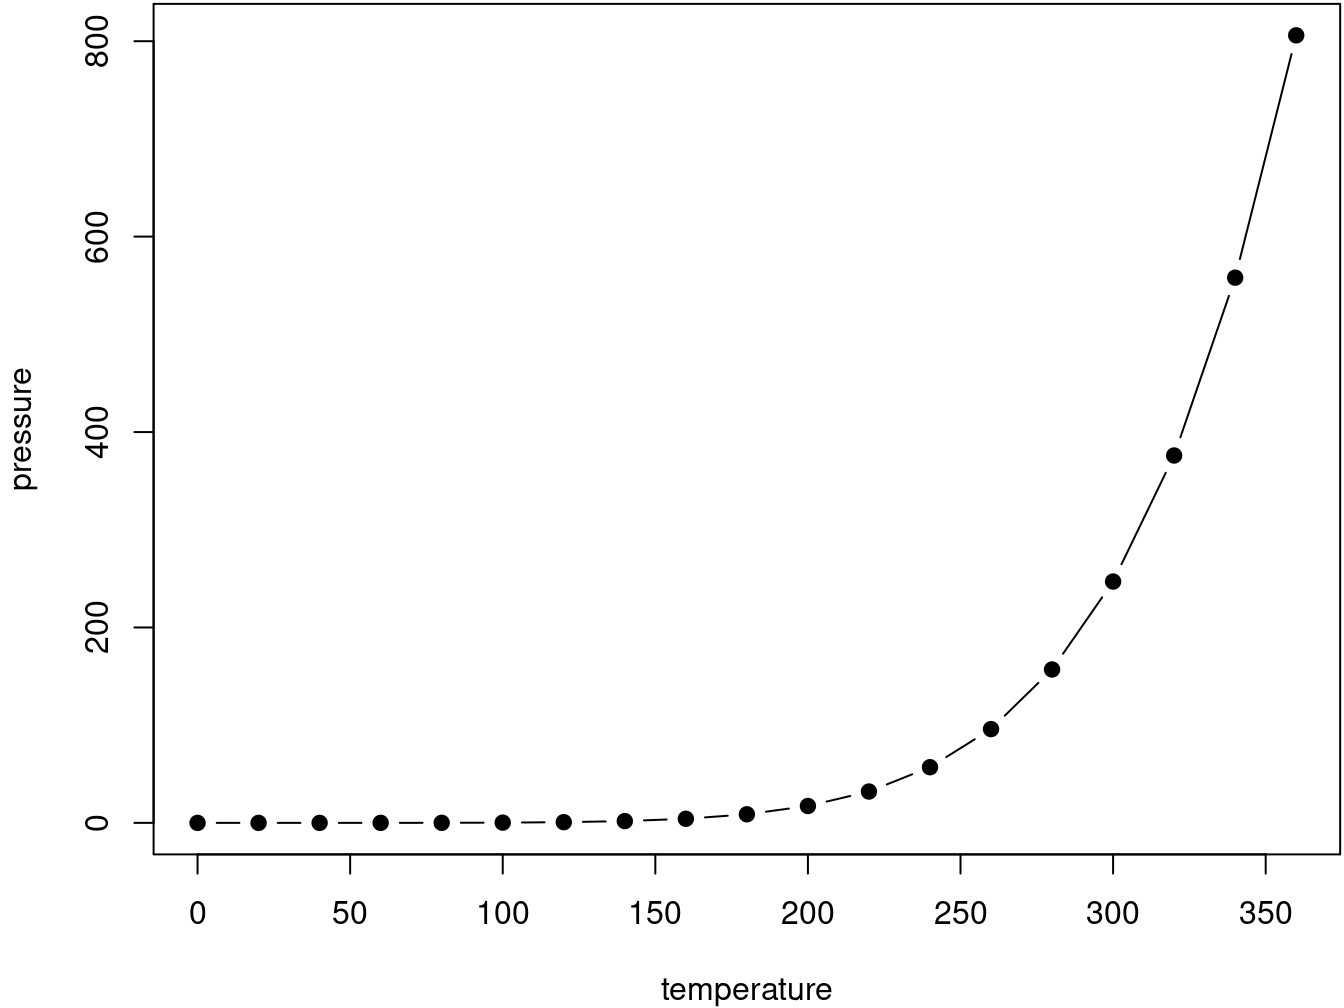
\includegraphics[width=0.8\linewidth]{data-science-practices-1_files/figure-latex/nice-fig-1} 

}

\caption{Here is a nice figure!}\label{fig:nice-fig}
\end{figure}

Reference a figure by its code chunk label with the \texttt{fig:} prefix, e.g., see Figure \ref{fig:nice-fig}. Similarly, you can reference tables generated from \texttt{knitr::kable()}, e.g., see Table \ref{tab:nice-tab}.

\begin{Shaded}
\begin{Highlighting}[]
\NormalTok{knitr}\OperatorTok{::}\KeywordTok{kable}\NormalTok{(}
  \KeywordTok{head}\NormalTok{(iris, }\DecValTok{20}\NormalTok{), }\DataTypeTok{caption =} \StringTok{\textquotesingle{}Here is a nice table!\textquotesingle{}}\NormalTok{,}
  \DataTypeTok{booktabs =} \OtherTok{TRUE}
\NormalTok{)}
\end{Highlighting}
\end{Shaded}

\begin{table}

\caption{\label{tab:nice-tab}Here is a nice table!}
\centering
\begin{tabular}[t]{rrrrl}
\toprule
Sepal.Length & Sepal.Width & Petal.Length & Petal.Width & Species\\
\midrule
5.1 & 3.5 & 1.4 & 0.2 & setosa\\
4.9 & 3.0 & 1.4 & 0.2 & setosa\\
4.7 & 3.2 & 1.3 & 0.2 & setosa\\
4.6 & 3.1 & 1.5 & 0.2 & setosa\\
5.0 & 3.6 & 1.4 & 0.2 & setosa\\
\addlinespace
5.4 & 3.9 & 1.7 & 0.4 & setosa\\
4.6 & 3.4 & 1.4 & 0.3 & setosa\\
5.0 & 3.4 & 1.5 & 0.2 & setosa\\
4.4 & 2.9 & 1.4 & 0.2 & setosa\\
4.9 & 3.1 & 1.5 & 0.1 & setosa\\
\addlinespace
5.4 & 3.7 & 1.5 & 0.2 & setosa\\
4.8 & 3.4 & 1.6 & 0.2 & setosa\\
4.8 & 3.0 & 1.4 & 0.1 & setosa\\
4.3 & 3.0 & 1.1 & 0.1 & setosa\\
5.8 & 4.0 & 1.2 & 0.2 & setosa\\
\addlinespace
5.7 & 4.4 & 1.5 & 0.4 & setosa\\
5.4 & 3.9 & 1.3 & 0.4 & setosa\\
5.1 & 3.5 & 1.4 & 0.3 & setosa\\
5.7 & 3.8 & 1.7 & 0.3 & setosa\\
5.1 & 3.8 & 1.5 & 0.3 & setosa\\
\bottomrule
\end{tabular}
\end{table}

You can write citations, too. For example, we are using the \textbf{bookdown} package \citep{R-bookdown} in this sample book, which was built on top of R Markdown and \textbf{knitr} \citep{xie2015}.

\hypertarget{acknowledgements}{%
\chapter{Acknowledgements}\label{acknowledgements}}

The authors thank all our colleauges for the discussions and experiences about data science that lead to this book. At OUHSC, this includes
\href{https://github.com/adrose}{@adrose},
\href{https://github.com/aggie-dbc}{@aggie-dbc},
\href{https://github.com/ARPeters}{@ARPeters},
\href{https://github.com/Ashley-Jorgensen}{@Ashley-Jorgensen},
\href{https://github.com/athumann}{@athumann},
\href{https://github.com/atreat1}{@atreat1},
\href{https://github.com/caston60}{@caston60},
\href{https://github.com/chanukyalakamsani}{@chanukyalakamsani},
\href{https://github.com/CWilliamsOUHSC}{@CWilliamsOUHSC},
\href{https://github.com/DavidBard}{@DavidBard},
\href{https://github.com/evoss1}{@evoss1},
\href{https://github.com/genevamarshall}{@genevamarshall},
\href{https://github.com/Maleeha}{@Maleeha},
\href{https://github.com/man9472}{@man9472},
\href{https://github.com/rmatkins}{@rmatkins},
\href{https://github.com/sbohora}{@sbohora},
\href{https://github.com/vimleshbavadiya}{@vimleshbavadiya},
\href{https://github.com/waleboro}{@waleboro},
\href{https://github.com/YuiYamaoka}{@YuiYamaoka},
\href{https://github.com/yutiantang}{@yutiantang}.

Outside the OUHSC, this includes

\href{https://github.com/andkov}{@andkov},
\href{https://github.com/ben519}{@ben519},
\href{https://github.com/cscherrer}{@cscherrer},
\href{https://github.com/cmodzelewski}{@cmodzelewski},
\href{https://github.com/jimquallen}{@jimquallen},
\href{https://github.com/mhunter1}{@mhunter1},
\href{https://github.com/probinso}{@probinso},
\href{https://github.com/russelljonas}{@russelljonas}, and
\href{https://github.com/spopovych}{@spopovych}.

\backmatter
  \bibliography{book.bib,packages.bib}

\end{document}
